%\begin{figure}[H]
%	\centering
%	% This file was created by matlab2tikz.
%
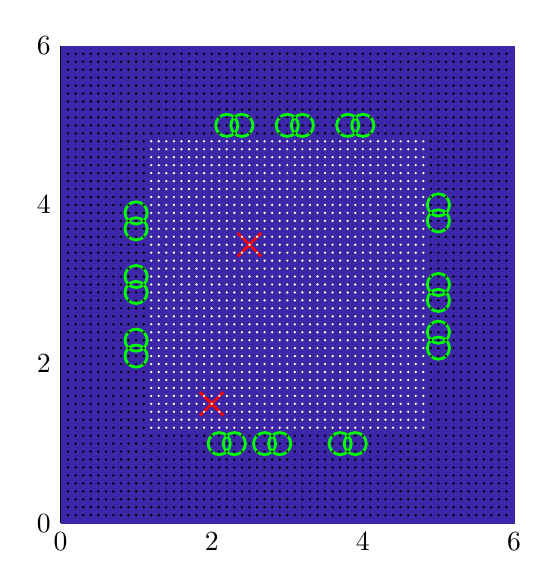
\begin{tikzpicture}

\begin{axis}[%
width=0.475\textwidth,
height=0.5\textwidth,
at={(0\textwidth,0\textwidth)},
scale only axis,
xmin=-0,
xmax=6,
ymin=-0,
ymax=6,
axis background/.style={fill=white},
axis x line*=bottom,
axis y line*=left
]

\addplot[%
surf,
shader=interp, colormap={mymap}{[1pt] rgb(0pt)=(0.239216,0.14902,0.658824); rgb(1pt)=(0.239216,0.14902,0.658824)}, mesh/rows=6]
table[row sep=crcr, point meta=\thisrow{c}] {%
%
x	y	c\\
0	0	0\\
0	1.2	0\\
0	2.4	0\\
0	3.6	0\\
0	4.8	0\\
0	6	0\\
1.2	0	0\\
1.2	1.2	0\\
1.2	2.4	0\\
1.2	3.6	0\\
1.2	4.8	0\\
1.2	6	0\\
2.4	0	0\\
2.4	1.2	0\\
2.4	2.4	0\\
2.4	3.6	0\\
2.4	4.8	0\\
2.4	6	0\\
3.6	0	0\\
3.6	1.2	0\\
3.6	2.4	0\\
3.6	3.6	0\\
3.6	4.8	0\\
3.6	6	0\\
4.8	0	0\\
4.8	1.2	0\\
4.8	2.4	0\\
4.8	3.6	0\\
4.8	4.8	0\\
4.8	6	0\\
6	0	0\\
6	1.2	0\\
6	2.4	0\\
6	3.6	0\\
6	4.8	0\\
6	6	0\\
};
\addplot [color=green, line width=1.0pt, draw=none, mark size=4.0pt, mark=o, mark options={solid, green}, forget plot]
  table[row sep=crcr]{%
2.1	1\\
2.3	1\\
2.7	1\\
2.9	1\\
3.7	1\\
3.9	1\\
5	2.2\\
5	2.4\\
5	2.8\\
5	3\\
5	3.8\\
5	4\\
2.2	5\\
2.4	5\\
3	5\\
3.2	5\\
3.8	5\\
4	5\\
1	2.1\\
1	2.3\\
1	2.9\\
1	3.1\\
1	3.7\\
1	3.9\\
};
\addplot [color=red, line width=1.0pt, draw=none, mark size=6.0pt, mark=x, mark options={solid, red}, forget plot]
  table[row sep=crcr]{%
2	1.5\\
2.5	3.5\\
};
\addplot [color=black, draw=none, mark size=0.2pt, mark=*, mark options={solid, black}, forget plot]
  table[row sep=crcr]{%
0.1	0.1\\
0.1	0.2\\
0.1	0.3\\
0.1	0.4\\
0.1	0.5\\
0.1	0.6\\
0.1	0.7\\
0.1	0.8\\
0.1	0.9\\
0.1	1\\
0.1	1.1\\
0.1	1.2\\
0.1	1.3\\
0.1	1.4\\
0.1	1.5\\
0.1	1.6\\
0.1	1.7\\
0.1	1.8\\
0.1	1.9\\
0.1	2\\
0.1	2.1\\
0.1	2.2\\
0.1	2.3\\
0.1	2.4\\
0.1	2.5\\
0.1	2.6\\
0.1	2.7\\
0.1	2.8\\
0.1	2.9\\
0.1	3\\
0.1	3.1\\
0.1	3.2\\
0.1	3.3\\
0.1	3.4\\
0.1	3.5\\
0.1	3.6\\
0.1	3.7\\
0.1	3.8\\
0.1	3.9\\
0.1	4\\
0.1	4.1\\
0.1	4.2\\
0.1	4.3\\
0.1	4.4\\
0.1	4.5\\
0.1	4.6\\
0.1	4.7\\
0.1	4.8\\
0.1	4.9\\
0.1	5\\
0.1	5.1\\
0.1	5.2\\
0.1	5.3\\
0.1	5.4\\
0.1	5.5\\
0.1	5.6\\
0.1	5.7\\
0.1	5.8\\
0.1	5.9\\
};
\addplot [color=black, draw=none, mark size=0.2pt, mark=*, mark options={solid, black}, forget plot]
  table[row sep=crcr]{%
0.2	0.1\\
0.2	0.2\\
0.2	0.3\\
0.2	0.4\\
0.2	0.5\\
0.2	0.6\\
0.2	0.7\\
0.2	0.8\\
0.2	0.9\\
0.2	1\\
0.2	1.1\\
0.2	1.2\\
0.2	1.3\\
0.2	1.4\\
0.2	1.5\\
0.2	1.6\\
0.2	1.7\\
0.2	1.8\\
0.2	1.9\\
0.2	2\\
0.2	2.1\\
0.2	2.2\\
0.2	2.3\\
0.2	2.4\\
0.2	2.5\\
0.2	2.6\\
0.2	2.7\\
0.2	2.8\\
0.2	2.9\\
0.2	3\\
0.2	3.1\\
0.2	3.2\\
0.2	3.3\\
0.2	3.4\\
0.2	3.5\\
0.2	3.6\\
0.2	3.7\\
0.2	3.8\\
0.2	3.9\\
0.2	4\\
0.2	4.1\\
0.2	4.2\\
0.2	4.3\\
0.2	4.4\\
0.2	4.5\\
0.2	4.6\\
0.2	4.7\\
0.2	4.8\\
0.2	4.9\\
0.2	5\\
0.2	5.1\\
0.2	5.2\\
0.2	5.3\\
0.2	5.4\\
0.2	5.5\\
0.2	5.6\\
0.2	5.7\\
0.2	5.8\\
0.2	5.9\\
};
\addplot [color=black, draw=none, mark size=0.2pt, mark=*, mark options={solid, black}, forget plot]
  table[row sep=crcr]{%
0.3	0.1\\
0.3	0.2\\
0.3	0.3\\
0.3	0.4\\
0.3	0.5\\
0.3	0.6\\
0.3	0.7\\
0.3	0.8\\
0.3	0.9\\
0.3	1\\
0.3	1.1\\
0.3	1.2\\
0.3	1.3\\
0.3	1.4\\
0.3	1.5\\
0.3	1.6\\
0.3	1.7\\
0.3	1.8\\
0.3	1.9\\
0.3	2\\
0.3	2.1\\
0.3	2.2\\
0.3	2.3\\
0.3	2.4\\
0.3	2.5\\
0.3	2.6\\
0.3	2.7\\
0.3	2.8\\
0.3	2.9\\
0.3	3\\
0.3	3.1\\
0.3	3.2\\
0.3	3.3\\
0.3	3.4\\
0.3	3.5\\
0.3	3.6\\
0.3	3.7\\
0.3	3.8\\
0.3	3.9\\
0.3	4\\
0.3	4.1\\
0.3	4.2\\
0.3	4.3\\
0.3	4.4\\
0.3	4.5\\
0.3	4.6\\
0.3	4.7\\
0.3	4.8\\
0.3	4.9\\
0.3	5\\
0.3	5.1\\
0.3	5.2\\
0.3	5.3\\
0.3	5.4\\
0.3	5.5\\
0.3	5.6\\
0.3	5.7\\
0.3	5.8\\
0.3	5.9\\
};
\addplot [color=black, draw=none, mark size=0.2pt, mark=*, mark options={solid, black}, forget plot]
  table[row sep=crcr]{%
0.4	0.1\\
0.4	0.2\\
0.4	0.3\\
0.4	0.4\\
0.4	0.5\\
0.4	0.6\\
0.4	0.7\\
0.4	0.8\\
0.4	0.9\\
0.4	1\\
0.4	1.1\\
0.4	1.2\\
0.4	1.3\\
0.4	1.4\\
0.4	1.5\\
0.4	1.6\\
0.4	1.7\\
0.4	1.8\\
0.4	1.9\\
0.4	2\\
0.4	2.1\\
0.4	2.2\\
0.4	2.3\\
0.4	2.4\\
0.4	2.5\\
0.4	2.6\\
0.4	2.7\\
0.4	2.8\\
0.4	2.9\\
0.4	3\\
0.4	3.1\\
0.4	3.2\\
0.4	3.3\\
0.4	3.4\\
0.4	3.5\\
0.4	3.6\\
0.4	3.7\\
0.4	3.8\\
0.4	3.9\\
0.4	4\\
0.4	4.1\\
0.4	4.2\\
0.4	4.3\\
0.4	4.4\\
0.4	4.5\\
0.4	4.6\\
0.4	4.7\\
0.4	4.8\\
0.4	4.9\\
0.4	5\\
0.4	5.1\\
0.4	5.2\\
0.4	5.3\\
0.4	5.4\\
0.4	5.5\\
0.4	5.6\\
0.4	5.7\\
0.4	5.8\\
0.4	5.9\\
};
\addplot [color=black, draw=none, mark size=0.2pt, mark=*, mark options={solid, black}, forget plot]
  table[row sep=crcr]{%
0.5	0.1\\
0.5	0.2\\
0.5	0.3\\
0.5	0.4\\
0.5	0.5\\
0.5	0.6\\
0.5	0.7\\
0.5	0.8\\
0.5	0.9\\
0.5	1\\
0.5	1.1\\
0.5	1.2\\
0.5	1.3\\
0.5	1.4\\
0.5	1.5\\
0.5	1.6\\
0.5	1.7\\
0.5	1.8\\
0.5	1.9\\
0.5	2\\
0.5	2.1\\
0.5	2.2\\
0.5	2.3\\
0.5	2.4\\
0.5	2.5\\
0.5	2.6\\
0.5	2.7\\
0.5	2.8\\
0.5	2.9\\
0.5	3\\
0.5	3.1\\
0.5	3.2\\
0.5	3.3\\
0.5	3.4\\
0.5	3.5\\
0.5	3.6\\
0.5	3.7\\
0.5	3.8\\
0.5	3.9\\
0.5	4\\
0.5	4.1\\
0.5	4.2\\
0.5	4.3\\
0.5	4.4\\
0.5	4.5\\
0.5	4.6\\
0.5	4.7\\
0.5	4.8\\
0.5	4.9\\
0.5	5\\
0.5	5.1\\
0.5	5.2\\
0.5	5.3\\
0.5	5.4\\
0.5	5.5\\
0.5	5.6\\
0.5	5.7\\
0.5	5.8\\
0.5	5.9\\
};
\addplot [color=black, draw=none, mark size=0.2pt, mark=*, mark options={solid, black}, forget plot]
  table[row sep=crcr]{%
0.6	0.1\\
0.6	0.2\\
0.6	0.3\\
0.6	0.4\\
0.6	0.5\\
0.6	0.6\\
0.6	0.7\\
0.6	0.8\\
0.6	0.9\\
0.6	1\\
0.6	1.1\\
0.6	1.2\\
0.6	1.3\\
0.6	1.4\\
0.6	1.5\\
0.6	1.6\\
0.6	1.7\\
0.6	1.8\\
0.6	1.9\\
0.6	2\\
0.6	2.1\\
0.6	2.2\\
0.6	2.3\\
0.6	2.4\\
0.6	2.5\\
0.6	2.6\\
0.6	2.7\\
0.6	2.8\\
0.6	2.9\\
0.6	3\\
0.6	3.1\\
0.6	3.2\\
0.6	3.3\\
0.6	3.4\\
0.6	3.5\\
0.6	3.6\\
0.6	3.7\\
0.6	3.8\\
0.6	3.9\\
0.6	4\\
0.6	4.1\\
0.6	4.2\\
0.6	4.3\\
0.6	4.4\\
0.6	4.5\\
0.6	4.6\\
0.6	4.7\\
0.6	4.8\\
0.6	4.9\\
0.6	5\\
0.6	5.1\\
0.6	5.2\\
0.6	5.3\\
0.6	5.4\\
0.6	5.5\\
0.6	5.6\\
0.6	5.7\\
0.6	5.8\\
0.6	5.9\\
};
\addplot [color=black, draw=none, mark size=0.2pt, mark=*, mark options={solid, black}, forget plot]
  table[row sep=crcr]{%
0.7	0.1\\
0.7	0.2\\
0.7	0.3\\
0.7	0.4\\
0.7	0.5\\
0.7	0.6\\
0.7	0.7\\
0.7	0.8\\
0.7	0.9\\
0.7	1\\
0.7	1.1\\
0.7	1.2\\
0.7	1.3\\
0.7	1.4\\
0.7	1.5\\
0.7	1.6\\
0.7	1.7\\
0.7	1.8\\
0.7	1.9\\
0.7	2\\
0.7	2.1\\
0.7	2.2\\
0.7	2.3\\
0.7	2.4\\
0.7	2.5\\
0.7	2.6\\
0.7	2.7\\
0.7	2.8\\
0.7	2.9\\
0.7	3\\
0.7	3.1\\
0.7	3.2\\
0.7	3.3\\
0.7	3.4\\
0.7	3.5\\
0.7	3.6\\
0.7	3.7\\
0.7	3.8\\
0.7	3.9\\
0.7	4\\
0.7	4.1\\
0.7	4.2\\
0.7	4.3\\
0.7	4.4\\
0.7	4.5\\
0.7	4.6\\
0.7	4.7\\
0.7	4.8\\
0.7	4.9\\
0.7	5\\
0.7	5.1\\
0.7	5.2\\
0.7	5.3\\
0.7	5.4\\
0.7	5.5\\
0.7	5.6\\
0.7	5.7\\
0.7	5.8\\
0.7	5.9\\
};
\addplot [color=black, draw=none, mark size=0.2pt, mark=*, mark options={solid, black}, forget plot]
  table[row sep=crcr]{%
0.8	0.1\\
0.8	0.2\\
0.8	0.3\\
0.8	0.4\\
0.8	0.5\\
0.8	0.6\\
0.8	0.7\\
0.8	0.8\\
0.8	0.9\\
0.8	1\\
0.8	1.1\\
0.8	1.2\\
0.8	1.3\\
0.8	1.4\\
0.8	1.5\\
0.8	1.6\\
0.8	1.7\\
0.8	1.8\\
0.8	1.9\\
0.8	2\\
0.8	2.1\\
0.8	2.2\\
0.8	2.3\\
0.8	2.4\\
0.8	2.5\\
0.8	2.6\\
0.8	2.7\\
0.8	2.8\\
0.8	2.9\\
0.8	3\\
0.8	3.1\\
0.8	3.2\\
0.8	3.3\\
0.8	3.4\\
0.8	3.5\\
0.8	3.6\\
0.8	3.7\\
0.8	3.8\\
0.8	3.9\\
0.8	4\\
0.8	4.1\\
0.8	4.2\\
0.8	4.3\\
0.8	4.4\\
0.8	4.5\\
0.8	4.6\\
0.8	4.7\\
0.8	4.8\\
0.8	4.9\\
0.8	5\\
0.8	5.1\\
0.8	5.2\\
0.8	5.3\\
0.8	5.4\\
0.8	5.5\\
0.8	5.6\\
0.8	5.7\\
0.8	5.8\\
0.8	5.9\\
};
\addplot [color=black, draw=none, mark size=0.2pt, mark=*, mark options={solid, black}, forget plot]
  table[row sep=crcr]{%
0.9	0.1\\
0.9	0.2\\
0.9	0.3\\
0.9	0.4\\
0.9	0.5\\
0.9	0.6\\
0.9	0.7\\
0.9	0.8\\
0.9	0.9\\
0.9	1\\
0.9	1.1\\
0.9	1.2\\
0.9	1.3\\
0.9	1.4\\
0.9	1.5\\
0.9	1.6\\
0.9	1.7\\
0.9	1.8\\
0.9	1.9\\
0.9	2\\
0.9	2.1\\
0.9	2.2\\
0.9	2.3\\
0.9	2.4\\
0.9	2.5\\
0.9	2.6\\
0.9	2.7\\
0.9	2.8\\
0.9	2.9\\
0.9	3\\
0.9	3.1\\
0.9	3.2\\
0.9	3.3\\
0.9	3.4\\
0.9	3.5\\
0.9	3.6\\
0.9	3.7\\
0.9	3.8\\
0.9	3.9\\
0.9	4\\
0.9	4.1\\
0.9	4.2\\
0.9	4.3\\
0.9	4.4\\
0.9	4.5\\
0.9	4.6\\
0.9	4.7\\
0.9	4.8\\
0.9	4.9\\
0.9	5\\
0.9	5.1\\
0.9	5.2\\
0.9	5.3\\
0.9	5.4\\
0.9	5.5\\
0.9	5.6\\
0.9	5.7\\
0.9	5.8\\
0.9	5.9\\
};
\addplot [color=black, draw=none, mark size=0.2pt, mark=*, mark options={solid, black}, forget plot]
  table[row sep=crcr]{%
1	0.1\\
1	0.2\\
1	0.3\\
1	0.4\\
1	0.5\\
1	0.6\\
1	0.7\\
1	0.8\\
1	0.9\\
1	1\\
1	1.1\\
1	1.2\\
1	1.3\\
1	1.4\\
1	1.5\\
1	1.6\\
1	1.7\\
1	1.8\\
1	1.9\\
1	2\\
1	2.1\\
1	2.2\\
1	2.3\\
1	2.4\\
1	2.5\\
1	2.6\\
1	2.7\\
1	2.8\\
1	2.9\\
1	3\\
1	3.1\\
1	3.2\\
1	3.3\\
1	3.4\\
1	3.5\\
1	3.6\\
1	3.7\\
1	3.8\\
1	3.9\\
1	4\\
1	4.1\\
1	4.2\\
1	4.3\\
1	4.4\\
1	4.5\\
1	4.6\\
1	4.7\\
1	4.8\\
1	4.9\\
1	5\\
1	5.1\\
1	5.2\\
1	5.3\\
1	5.4\\
1	5.5\\
1	5.6\\
1	5.7\\
1	5.8\\
1	5.9\\
};
\addplot [color=black, draw=none, mark size=0.2pt, mark=*, mark options={solid, black}, forget plot]
  table[row sep=crcr]{%
1.1	0.1\\
1.1	0.2\\
1.1	0.3\\
1.1	0.4\\
1.1	0.5\\
1.1	0.6\\
1.1	0.7\\
1.1	0.8\\
1.1	0.9\\
1.1	1\\
1.1	1.1\\
1.1	1.2\\
1.1	1.3\\
1.1	1.4\\
1.1	1.5\\
1.1	1.6\\
1.1	1.7\\
1.1	1.8\\
1.1	1.9\\
1.1	2\\
1.1	2.1\\
1.1	2.2\\
1.1	2.3\\
1.1	2.4\\
1.1	2.5\\
1.1	2.6\\
1.1	2.7\\
1.1	2.8\\
1.1	2.9\\
1.1	3\\
1.1	3.1\\
1.1	3.2\\
1.1	3.3\\
1.1	3.4\\
1.1	3.5\\
1.1	3.6\\
1.1	3.7\\
1.1	3.8\\
1.1	3.9\\
1.1	4\\
1.1	4.1\\
1.1	4.2\\
1.1	4.3\\
1.1	4.4\\
1.1	4.5\\
1.1	4.6\\
1.1	4.7\\
1.1	4.8\\
1.1	4.9\\
1.1	5\\
1.1	5.1\\
1.1	5.2\\
1.1	5.3\\
1.1	5.4\\
1.1	5.5\\
1.1	5.6\\
1.1	5.7\\
1.1	5.8\\
1.1	5.9\\
};
\addplot [color=black, draw=none, mark size=0.2pt, mark=*, mark options={solid, black}, forget plot]
  table[row sep=crcr]{%
1.2	0.1\\
1.2	0.2\\
1.2	0.3\\
1.2	0.4\\
1.2	0.5\\
1.2	0.6\\
1.2	0.7\\
1.2	0.8\\
1.2	0.9\\
1.2	1\\
1.2	1.1\\
1.2	1.2\\
1.2	1.3\\
1.2	1.4\\
1.2	1.5\\
1.2	1.6\\
1.2	1.7\\
1.2	1.8\\
1.2	1.9\\
1.2	2\\
1.2	2.1\\
1.2	2.2\\
1.2	2.3\\
1.2	2.4\\
1.2	2.5\\
1.2	2.6\\
1.2	2.7\\
1.2	2.8\\
1.2	2.9\\
1.2	3\\
1.2	3.1\\
1.2	3.2\\
1.2	3.3\\
1.2	3.4\\
1.2	3.5\\
1.2	3.6\\
1.2	3.7\\
1.2	3.8\\
1.2	3.9\\
1.2	4\\
1.2	4.1\\
1.2	4.2\\
1.2	4.3\\
1.2	4.4\\
1.2	4.5\\
1.2	4.6\\
1.2	4.7\\
1.2	4.8\\
1.2	4.9\\
1.2	5\\
1.2	5.1\\
1.2	5.2\\
1.2	5.3\\
1.2	5.4\\
1.2	5.5\\
1.2	5.6\\
1.2	5.7\\
1.2	5.8\\
1.2	5.9\\
};
\addplot [color=black, draw=none, mark size=0.2pt, mark=*, mark options={solid, black}, forget plot]
  table[row sep=crcr]{%
1.3	0.1\\
1.3	0.2\\
1.3	0.3\\
1.3	0.4\\
1.3	0.5\\
1.3	0.6\\
1.3	0.7\\
1.3	0.8\\
1.3	0.9\\
1.3	1\\
1.3	1.1\\
1.3	1.2\\
1.3	1.3\\
1.3	1.4\\
1.3	1.5\\
1.3	1.6\\
1.3	1.7\\
1.3	1.8\\
1.3	1.9\\
1.3	2\\
1.3	2.1\\
1.3	2.2\\
1.3	2.3\\
1.3	2.4\\
1.3	2.5\\
1.3	2.6\\
1.3	2.7\\
1.3	2.8\\
1.3	2.9\\
1.3	3\\
1.3	3.1\\
1.3	3.2\\
1.3	3.3\\
1.3	3.4\\
1.3	3.5\\
1.3	3.6\\
1.3	3.7\\
1.3	3.8\\
1.3	3.9\\
1.3	4\\
1.3	4.1\\
1.3	4.2\\
1.3	4.3\\
1.3	4.4\\
1.3	4.5\\
1.3	4.6\\
1.3	4.7\\
1.3	4.8\\
1.3	4.9\\
1.3	5\\
1.3	5.1\\
1.3	5.2\\
1.3	5.3\\
1.3	5.4\\
1.3	5.5\\
1.3	5.6\\
1.3	5.7\\
1.3	5.8\\
1.3	5.9\\
};
\addplot [color=black, draw=none, mark size=0.2pt, mark=*, mark options={solid, black}, forget plot]
  table[row sep=crcr]{%
1.4	0.1\\
1.4	0.2\\
1.4	0.3\\
1.4	0.4\\
1.4	0.5\\
1.4	0.6\\
1.4	0.7\\
1.4	0.8\\
1.4	0.9\\
1.4	1\\
1.4	1.1\\
1.4	1.2\\
1.4	1.3\\
1.4	1.4\\
1.4	1.5\\
1.4	1.6\\
1.4	1.7\\
1.4	1.8\\
1.4	1.9\\
1.4	2\\
1.4	2.1\\
1.4	2.2\\
1.4	2.3\\
1.4	2.4\\
1.4	2.5\\
1.4	2.6\\
1.4	2.7\\
1.4	2.8\\
1.4	2.9\\
1.4	3\\
1.4	3.1\\
1.4	3.2\\
1.4	3.3\\
1.4	3.4\\
1.4	3.5\\
1.4	3.6\\
1.4	3.7\\
1.4	3.8\\
1.4	3.9\\
1.4	4\\
1.4	4.1\\
1.4	4.2\\
1.4	4.3\\
1.4	4.4\\
1.4	4.5\\
1.4	4.6\\
1.4	4.7\\
1.4	4.8\\
1.4	4.9\\
1.4	5\\
1.4	5.1\\
1.4	5.2\\
1.4	5.3\\
1.4	5.4\\
1.4	5.5\\
1.4	5.6\\
1.4	5.7\\
1.4	5.8\\
1.4	5.9\\
};
\addplot [color=black, draw=none, mark size=0.2pt, mark=*, mark options={solid, black}, forget plot]
  table[row sep=crcr]{%
1.5	0.1\\
1.5	0.2\\
1.5	0.3\\
1.5	0.4\\
1.5	0.5\\
1.5	0.6\\
1.5	0.7\\
1.5	0.8\\
1.5	0.9\\
1.5	1\\
1.5	1.1\\
1.5	1.2\\
1.5	1.3\\
1.5	1.4\\
1.5	1.5\\
1.5	1.6\\
1.5	1.7\\
1.5	1.8\\
1.5	1.9\\
1.5	2\\
1.5	2.1\\
1.5	2.2\\
1.5	2.3\\
1.5	2.4\\
1.5	2.5\\
1.5	2.6\\
1.5	2.7\\
1.5	2.8\\
1.5	2.9\\
1.5	3\\
1.5	3.1\\
1.5	3.2\\
1.5	3.3\\
1.5	3.4\\
1.5	3.5\\
1.5	3.6\\
1.5	3.7\\
1.5	3.8\\
1.5	3.9\\
1.5	4\\
1.5	4.1\\
1.5	4.2\\
1.5	4.3\\
1.5	4.4\\
1.5	4.5\\
1.5	4.6\\
1.5	4.7\\
1.5	4.8\\
1.5	4.9\\
1.5	5\\
1.5	5.1\\
1.5	5.2\\
1.5	5.3\\
1.5	5.4\\
1.5	5.5\\
1.5	5.6\\
1.5	5.7\\
1.5	5.8\\
1.5	5.9\\
};
\addplot [color=black, draw=none, mark size=0.2pt, mark=*, mark options={solid, black}, forget plot]
  table[row sep=crcr]{%
1.6	0.1\\
1.6	0.2\\
1.6	0.3\\
1.6	0.4\\
1.6	0.5\\
1.6	0.6\\
1.6	0.7\\
1.6	0.8\\
1.6	0.9\\
1.6	1\\
1.6	1.1\\
1.6	1.2\\
1.6	1.3\\
1.6	1.4\\
1.6	1.5\\
1.6	1.6\\
1.6	1.7\\
1.6	1.8\\
1.6	1.9\\
1.6	2\\
1.6	2.1\\
1.6	2.2\\
1.6	2.3\\
1.6	2.4\\
1.6	2.5\\
1.6	2.6\\
1.6	2.7\\
1.6	2.8\\
1.6	2.9\\
1.6	3\\
1.6	3.1\\
1.6	3.2\\
1.6	3.3\\
1.6	3.4\\
1.6	3.5\\
1.6	3.6\\
1.6	3.7\\
1.6	3.8\\
1.6	3.9\\
1.6	4\\
1.6	4.1\\
1.6	4.2\\
1.6	4.3\\
1.6	4.4\\
1.6	4.5\\
1.6	4.6\\
1.6	4.7\\
1.6	4.8\\
1.6	4.9\\
1.6	5\\
1.6	5.1\\
1.6	5.2\\
1.6	5.3\\
1.6	5.4\\
1.6	5.5\\
1.6	5.6\\
1.6	5.7\\
1.6	5.8\\
1.6	5.9\\
};
\addplot [color=black, draw=none, mark size=0.2pt, mark=*, mark options={solid, black}, forget plot]
  table[row sep=crcr]{%
1.7	0.1\\
1.7	0.2\\
1.7	0.3\\
1.7	0.4\\
1.7	0.5\\
1.7	0.6\\
1.7	0.7\\
1.7	0.8\\
1.7	0.9\\
1.7	1\\
1.7	1.1\\
1.7	1.2\\
1.7	1.3\\
1.7	1.4\\
1.7	1.5\\
1.7	1.6\\
1.7	1.7\\
1.7	1.8\\
1.7	1.9\\
1.7	2\\
1.7	2.1\\
1.7	2.2\\
1.7	2.3\\
1.7	2.4\\
1.7	2.5\\
1.7	2.6\\
1.7	2.7\\
1.7	2.8\\
1.7	2.9\\
1.7	3\\
1.7	3.1\\
1.7	3.2\\
1.7	3.3\\
1.7	3.4\\
1.7	3.5\\
1.7	3.6\\
1.7	3.7\\
1.7	3.8\\
1.7	3.9\\
1.7	4\\
1.7	4.1\\
1.7	4.2\\
1.7	4.3\\
1.7	4.4\\
1.7	4.5\\
1.7	4.6\\
1.7	4.7\\
1.7	4.8\\
1.7	4.9\\
1.7	5\\
1.7	5.1\\
1.7	5.2\\
1.7	5.3\\
1.7	5.4\\
1.7	5.5\\
1.7	5.6\\
1.7	5.7\\
1.7	5.8\\
1.7	5.9\\
};
\addplot [color=black, draw=none, mark size=0.2pt, mark=*, mark options={solid, black}, forget plot]
  table[row sep=crcr]{%
1.8	0.1\\
1.8	0.2\\
1.8	0.3\\
1.8	0.4\\
1.8	0.5\\
1.8	0.6\\
1.8	0.7\\
1.8	0.8\\
1.8	0.9\\
1.8	1\\
1.8	1.1\\
1.8	1.2\\
1.8	1.3\\
1.8	1.4\\
1.8	1.5\\
1.8	1.6\\
1.8	1.7\\
1.8	1.8\\
1.8	1.9\\
1.8	2\\
1.8	2.1\\
1.8	2.2\\
1.8	2.3\\
1.8	2.4\\
1.8	2.5\\
1.8	2.6\\
1.8	2.7\\
1.8	2.8\\
1.8	2.9\\
1.8	3\\
1.8	3.1\\
1.8	3.2\\
1.8	3.3\\
1.8	3.4\\
1.8	3.5\\
1.8	3.6\\
1.8	3.7\\
1.8	3.8\\
1.8	3.9\\
1.8	4\\
1.8	4.1\\
1.8	4.2\\
1.8	4.3\\
1.8	4.4\\
1.8	4.5\\
1.8	4.6\\
1.8	4.7\\
1.8	4.8\\
1.8	4.9\\
1.8	5\\
1.8	5.1\\
1.8	5.2\\
1.8	5.3\\
1.8	5.4\\
1.8	5.5\\
1.8	5.6\\
1.8	5.7\\
1.8	5.8\\
1.8	5.9\\
};
\addplot [color=black, draw=none, mark size=0.2pt, mark=*, mark options={solid, black}, forget plot]
  table[row sep=crcr]{%
1.9	0.1\\
1.9	0.2\\
1.9	0.3\\
1.9	0.4\\
1.9	0.5\\
1.9	0.6\\
1.9	0.7\\
1.9	0.8\\
1.9	0.9\\
1.9	1\\
1.9	1.1\\
1.9	1.2\\
1.9	1.3\\
1.9	1.4\\
1.9	1.5\\
1.9	1.6\\
1.9	1.7\\
1.9	1.8\\
1.9	1.9\\
1.9	2\\
1.9	2.1\\
1.9	2.2\\
1.9	2.3\\
1.9	2.4\\
1.9	2.5\\
1.9	2.6\\
1.9	2.7\\
1.9	2.8\\
1.9	2.9\\
1.9	3\\
1.9	3.1\\
1.9	3.2\\
1.9	3.3\\
1.9	3.4\\
1.9	3.5\\
1.9	3.6\\
1.9	3.7\\
1.9	3.8\\
1.9	3.9\\
1.9	4\\
1.9	4.1\\
1.9	4.2\\
1.9	4.3\\
1.9	4.4\\
1.9	4.5\\
1.9	4.6\\
1.9	4.7\\
1.9	4.8\\
1.9	4.9\\
1.9	5\\
1.9	5.1\\
1.9	5.2\\
1.9	5.3\\
1.9	5.4\\
1.9	5.5\\
1.9	5.6\\
1.9	5.7\\
1.9	5.8\\
1.9	5.9\\
};
\addplot [color=black, draw=none, mark size=0.2pt, mark=*, mark options={solid, black}, forget plot]
  table[row sep=crcr]{%
2	0.1\\
2	0.2\\
2	0.3\\
2	0.4\\
2	0.5\\
2	0.6\\
2	0.7\\
2	0.8\\
2	0.9\\
2	1\\
2	1.1\\
2	1.2\\
2	1.3\\
2	1.4\\
2	1.5\\
2	1.6\\
2	1.7\\
2	1.8\\
2	1.9\\
2	2\\
2	2.1\\
2	2.2\\
2	2.3\\
2	2.4\\
2	2.5\\
2	2.6\\
2	2.7\\
2	2.8\\
2	2.9\\
2	3\\
2	3.1\\
2	3.2\\
2	3.3\\
2	3.4\\
2	3.5\\
2	3.6\\
2	3.7\\
2	3.8\\
2	3.9\\
2	4\\
2	4.1\\
2	4.2\\
2	4.3\\
2	4.4\\
2	4.5\\
2	4.6\\
2	4.7\\
2	4.8\\
2	4.9\\
2	5\\
2	5.1\\
2	5.2\\
2	5.3\\
2	5.4\\
2	5.5\\
2	5.6\\
2	5.7\\
2	5.8\\
2	5.9\\
};
\addplot [color=black, draw=none, mark size=0.2pt, mark=*, mark options={solid, black}, forget plot]
  table[row sep=crcr]{%
2.1	0.1\\
2.1	0.2\\
2.1	0.3\\
2.1	0.4\\
2.1	0.5\\
2.1	0.6\\
2.1	0.7\\
2.1	0.8\\
2.1	0.9\\
2.1	1\\
2.1	1.1\\
2.1	1.2\\
2.1	1.3\\
2.1	1.4\\
2.1	1.5\\
2.1	1.6\\
2.1	1.7\\
2.1	1.8\\
2.1	1.9\\
2.1	2\\
2.1	2.1\\
2.1	2.2\\
2.1	2.3\\
2.1	2.4\\
2.1	2.5\\
2.1	2.6\\
2.1	2.7\\
2.1	2.8\\
2.1	2.9\\
2.1	3\\
2.1	3.1\\
2.1	3.2\\
2.1	3.3\\
2.1	3.4\\
2.1	3.5\\
2.1	3.6\\
2.1	3.7\\
2.1	3.8\\
2.1	3.9\\
2.1	4\\
2.1	4.1\\
2.1	4.2\\
2.1	4.3\\
2.1	4.4\\
2.1	4.5\\
2.1	4.6\\
2.1	4.7\\
2.1	4.8\\
2.1	4.9\\
2.1	5\\
2.1	5.1\\
2.1	5.2\\
2.1	5.3\\
2.1	5.4\\
2.1	5.5\\
2.1	5.6\\
2.1	5.7\\
2.1	5.8\\
2.1	5.9\\
};
\addplot [color=black, draw=none, mark size=0.2pt, mark=*, mark options={solid, black}, forget plot]
  table[row sep=crcr]{%
2.2	0.1\\
2.2	0.2\\
2.2	0.3\\
2.2	0.4\\
2.2	0.5\\
2.2	0.6\\
2.2	0.7\\
2.2	0.8\\
2.2	0.9\\
2.2	1\\
2.2	1.1\\
2.2	1.2\\
2.2	1.3\\
2.2	1.4\\
2.2	1.5\\
2.2	1.6\\
2.2	1.7\\
2.2	1.8\\
2.2	1.9\\
2.2	2\\
2.2	2.1\\
2.2	2.2\\
2.2	2.3\\
2.2	2.4\\
2.2	2.5\\
2.2	2.6\\
2.2	2.7\\
2.2	2.8\\
2.2	2.9\\
2.2	3\\
2.2	3.1\\
2.2	3.2\\
2.2	3.3\\
2.2	3.4\\
2.2	3.5\\
2.2	3.6\\
2.2	3.7\\
2.2	3.8\\
2.2	3.9\\
2.2	4\\
2.2	4.1\\
2.2	4.2\\
2.2	4.3\\
2.2	4.4\\
2.2	4.5\\
2.2	4.6\\
2.2	4.7\\
2.2	4.8\\
2.2	4.9\\
2.2	5\\
2.2	5.1\\
2.2	5.2\\
2.2	5.3\\
2.2	5.4\\
2.2	5.5\\
2.2	5.6\\
2.2	5.7\\
2.2	5.8\\
2.2	5.9\\
};
\addplot [color=black, draw=none, mark size=0.2pt, mark=*, mark options={solid, black}, forget plot]
  table[row sep=crcr]{%
2.3	0.1\\
2.3	0.2\\
2.3	0.3\\
2.3	0.4\\
2.3	0.5\\
2.3	0.6\\
2.3	0.7\\
2.3	0.8\\
2.3	0.9\\
2.3	1\\
2.3	1.1\\
2.3	1.2\\
2.3	1.3\\
2.3	1.4\\
2.3	1.5\\
2.3	1.6\\
2.3	1.7\\
2.3	1.8\\
2.3	1.9\\
2.3	2\\
2.3	2.1\\
2.3	2.2\\
2.3	2.3\\
2.3	2.4\\
2.3	2.5\\
2.3	2.6\\
2.3	2.7\\
2.3	2.8\\
2.3	2.9\\
2.3	3\\
2.3	3.1\\
2.3	3.2\\
2.3	3.3\\
2.3	3.4\\
2.3	3.5\\
2.3	3.6\\
2.3	3.7\\
2.3	3.8\\
2.3	3.9\\
2.3	4\\
2.3	4.1\\
2.3	4.2\\
2.3	4.3\\
2.3	4.4\\
2.3	4.5\\
2.3	4.6\\
2.3	4.7\\
2.3	4.8\\
2.3	4.9\\
2.3	5\\
2.3	5.1\\
2.3	5.2\\
2.3	5.3\\
2.3	5.4\\
2.3	5.5\\
2.3	5.6\\
2.3	5.7\\
2.3	5.8\\
2.3	5.9\\
};
\addplot [color=black, draw=none, mark size=0.2pt, mark=*, mark options={solid, black}, forget plot]
  table[row sep=crcr]{%
2.4	0.1\\
2.4	0.2\\
2.4	0.3\\
2.4	0.4\\
2.4	0.5\\
2.4	0.6\\
2.4	0.7\\
2.4	0.8\\
2.4	0.9\\
2.4	1\\
2.4	1.1\\
2.4	1.2\\
2.4	1.3\\
2.4	1.4\\
2.4	1.5\\
2.4	1.6\\
2.4	1.7\\
2.4	1.8\\
2.4	1.9\\
2.4	2\\
2.4	2.1\\
2.4	2.2\\
2.4	2.3\\
2.4	2.4\\
2.4	2.5\\
2.4	2.6\\
2.4	2.7\\
2.4	2.8\\
2.4	2.9\\
2.4	3\\
2.4	3.1\\
2.4	3.2\\
2.4	3.3\\
2.4	3.4\\
2.4	3.5\\
2.4	3.6\\
2.4	3.7\\
2.4	3.8\\
2.4	3.9\\
2.4	4\\
2.4	4.1\\
2.4	4.2\\
2.4	4.3\\
2.4	4.4\\
2.4	4.5\\
2.4	4.6\\
2.4	4.7\\
2.4	4.8\\
2.4	4.9\\
2.4	5\\
2.4	5.1\\
2.4	5.2\\
2.4	5.3\\
2.4	5.4\\
2.4	5.5\\
2.4	5.6\\
2.4	5.7\\
2.4	5.8\\
2.4	5.9\\
};
\addplot [color=black, draw=none, mark size=0.2pt, mark=*, mark options={solid, black}, forget plot]
  table[row sep=crcr]{%
2.5	0.1\\
2.5	0.2\\
2.5	0.3\\
2.5	0.4\\
2.5	0.5\\
2.5	0.6\\
2.5	0.7\\
2.5	0.8\\
2.5	0.9\\
2.5	1\\
2.5	1.1\\
2.5	1.2\\
2.5	1.3\\
2.5	1.4\\
2.5	1.5\\
2.5	1.6\\
2.5	1.7\\
2.5	1.8\\
2.5	1.9\\
2.5	2\\
2.5	2.1\\
2.5	2.2\\
2.5	2.3\\
2.5	2.4\\
2.5	2.5\\
2.5	2.6\\
2.5	2.7\\
2.5	2.8\\
2.5	2.9\\
2.5	3\\
2.5	3.1\\
2.5	3.2\\
2.5	3.3\\
2.5	3.4\\
2.5	3.5\\
2.5	3.6\\
2.5	3.7\\
2.5	3.8\\
2.5	3.9\\
2.5	4\\
2.5	4.1\\
2.5	4.2\\
2.5	4.3\\
2.5	4.4\\
2.5	4.5\\
2.5	4.6\\
2.5	4.7\\
2.5	4.8\\
2.5	4.9\\
2.5	5\\
2.5	5.1\\
2.5	5.2\\
2.5	5.3\\
2.5	5.4\\
2.5	5.5\\
2.5	5.6\\
2.5	5.7\\
2.5	5.8\\
2.5	5.9\\
};
\addplot [color=black, draw=none, mark size=0.2pt, mark=*, mark options={solid, black}, forget plot]
  table[row sep=crcr]{%
2.6	0.1\\
2.6	0.2\\
2.6	0.3\\
2.6	0.4\\
2.6	0.5\\
2.6	0.6\\
2.6	0.7\\
2.6	0.8\\
2.6	0.9\\
2.6	1\\
2.6	1.1\\
2.6	1.2\\
2.6	1.3\\
2.6	1.4\\
2.6	1.5\\
2.6	1.6\\
2.6	1.7\\
2.6	1.8\\
2.6	1.9\\
2.6	2\\
2.6	2.1\\
2.6	2.2\\
2.6	2.3\\
2.6	2.4\\
2.6	2.5\\
2.6	2.6\\
2.6	2.7\\
2.6	2.8\\
2.6	2.9\\
2.6	3\\
2.6	3.1\\
2.6	3.2\\
2.6	3.3\\
2.6	3.4\\
2.6	3.5\\
2.6	3.6\\
2.6	3.7\\
2.6	3.8\\
2.6	3.9\\
2.6	4\\
2.6	4.1\\
2.6	4.2\\
2.6	4.3\\
2.6	4.4\\
2.6	4.5\\
2.6	4.6\\
2.6	4.7\\
2.6	4.8\\
2.6	4.9\\
2.6	5\\
2.6	5.1\\
2.6	5.2\\
2.6	5.3\\
2.6	5.4\\
2.6	5.5\\
2.6	5.6\\
2.6	5.7\\
2.6	5.8\\
2.6	5.9\\
};
\addplot [color=black, draw=none, mark size=0.2pt, mark=*, mark options={solid, black}, forget plot]
  table[row sep=crcr]{%
2.7	0.1\\
2.7	0.2\\
2.7	0.3\\
2.7	0.4\\
2.7	0.5\\
2.7	0.6\\
2.7	0.7\\
2.7	0.8\\
2.7	0.9\\
2.7	1\\
2.7	1.1\\
2.7	1.2\\
2.7	1.3\\
2.7	1.4\\
2.7	1.5\\
2.7	1.6\\
2.7	1.7\\
2.7	1.8\\
2.7	1.9\\
2.7	2\\
2.7	2.1\\
2.7	2.2\\
2.7	2.3\\
2.7	2.4\\
2.7	2.5\\
2.7	2.6\\
2.7	2.7\\
2.7	2.8\\
2.7	2.9\\
2.7	3\\
2.7	3.1\\
2.7	3.2\\
2.7	3.3\\
2.7	3.4\\
2.7	3.5\\
2.7	3.6\\
2.7	3.7\\
2.7	3.8\\
2.7	3.9\\
2.7	4\\
2.7	4.1\\
2.7	4.2\\
2.7	4.3\\
2.7	4.4\\
2.7	4.5\\
2.7	4.6\\
2.7	4.7\\
2.7	4.8\\
2.7	4.9\\
2.7	5\\
2.7	5.1\\
2.7	5.2\\
2.7	5.3\\
2.7	5.4\\
2.7	5.5\\
2.7	5.6\\
2.7	5.7\\
2.7	5.8\\
2.7	5.9\\
};
\addplot [color=black, draw=none, mark size=0.2pt, mark=*, mark options={solid, black}, forget plot]
  table[row sep=crcr]{%
2.8	0.1\\
2.8	0.2\\
2.8	0.3\\
2.8	0.4\\
2.8	0.5\\
2.8	0.6\\
2.8	0.7\\
2.8	0.8\\
2.8	0.9\\
2.8	1\\
2.8	1.1\\
2.8	1.2\\
2.8	1.3\\
2.8	1.4\\
2.8	1.5\\
2.8	1.6\\
2.8	1.7\\
2.8	1.8\\
2.8	1.9\\
2.8	2\\
2.8	2.1\\
2.8	2.2\\
2.8	2.3\\
2.8	2.4\\
2.8	2.5\\
2.8	2.6\\
2.8	2.7\\
2.8	2.8\\
2.8	2.9\\
2.8	3\\
2.8	3.1\\
2.8	3.2\\
2.8	3.3\\
2.8	3.4\\
2.8	3.5\\
2.8	3.6\\
2.8	3.7\\
2.8	3.8\\
2.8	3.9\\
2.8	4\\
2.8	4.1\\
2.8	4.2\\
2.8	4.3\\
2.8	4.4\\
2.8	4.5\\
2.8	4.6\\
2.8	4.7\\
2.8	4.8\\
2.8	4.9\\
2.8	5\\
2.8	5.1\\
2.8	5.2\\
2.8	5.3\\
2.8	5.4\\
2.8	5.5\\
2.8	5.6\\
2.8	5.7\\
2.8	5.8\\
2.8	5.9\\
};
\addplot [color=black, draw=none, mark size=0.2pt, mark=*, mark options={solid, black}, forget plot]
  table[row sep=crcr]{%
2.9	0.1\\
2.9	0.2\\
2.9	0.3\\
2.9	0.4\\
2.9	0.5\\
2.9	0.6\\
2.9	0.7\\
2.9	0.8\\
2.9	0.9\\
2.9	1\\
2.9	1.1\\
2.9	1.2\\
2.9	1.3\\
2.9	1.4\\
2.9	1.5\\
2.9	1.6\\
2.9	1.7\\
2.9	1.8\\
2.9	1.9\\
2.9	2\\
2.9	2.1\\
2.9	2.2\\
2.9	2.3\\
2.9	2.4\\
2.9	2.5\\
2.9	2.6\\
2.9	2.7\\
2.9	2.8\\
2.9	2.9\\
2.9	3\\
2.9	3.1\\
2.9	3.2\\
2.9	3.3\\
2.9	3.4\\
2.9	3.5\\
2.9	3.6\\
2.9	3.7\\
2.9	3.8\\
2.9	3.9\\
2.9	4\\
2.9	4.1\\
2.9	4.2\\
2.9	4.3\\
2.9	4.4\\
2.9	4.5\\
2.9	4.6\\
2.9	4.7\\
2.9	4.8\\
2.9	4.9\\
2.9	5\\
2.9	5.1\\
2.9	5.2\\
2.9	5.3\\
2.9	5.4\\
2.9	5.5\\
2.9	5.6\\
2.9	5.7\\
2.9	5.8\\
2.9	5.9\\
};
\addplot [color=black, draw=none, mark size=0.2pt, mark=*, mark options={solid, black}, forget plot]
  table[row sep=crcr]{%
3	0.1\\
3	0.2\\
3	0.3\\
3	0.4\\
3	0.5\\
3	0.6\\
3	0.7\\
3	0.8\\
3	0.9\\
3	1\\
3	1.1\\
3	1.2\\
3	1.3\\
3	1.4\\
3	1.5\\
3	1.6\\
3	1.7\\
3	1.8\\
3	1.9\\
3	2\\
3	2.1\\
3	2.2\\
3	2.3\\
3	2.4\\
3	2.5\\
3	2.6\\
3	2.7\\
3	2.8\\
3	2.9\\
3	3\\
3	3.1\\
3	3.2\\
3	3.3\\
3	3.4\\
3	3.5\\
3	3.6\\
3	3.7\\
3	3.8\\
3	3.9\\
3	4\\
3	4.1\\
3	4.2\\
3	4.3\\
3	4.4\\
3	4.5\\
3	4.6\\
3	4.7\\
3	4.8\\
3	4.9\\
3	5\\
3	5.1\\
3	5.2\\
3	5.3\\
3	5.4\\
3	5.5\\
3	5.6\\
3	5.7\\
3	5.8\\
3	5.9\\
};
\addplot [color=black, draw=none, mark size=0.2pt, mark=*, mark options={solid, black}, forget plot]
  table[row sep=crcr]{%
3.1	0.1\\
3.1	0.2\\
3.1	0.3\\
3.1	0.4\\
3.1	0.5\\
3.1	0.6\\
3.1	0.7\\
3.1	0.8\\
3.1	0.9\\
3.1	1\\
3.1	1.1\\
3.1	1.2\\
3.1	1.3\\
3.1	1.4\\
3.1	1.5\\
3.1	1.6\\
3.1	1.7\\
3.1	1.8\\
3.1	1.9\\
3.1	2\\
3.1	2.1\\
3.1	2.2\\
3.1	2.3\\
3.1	2.4\\
3.1	2.5\\
3.1	2.6\\
3.1	2.7\\
3.1	2.8\\
3.1	2.9\\
3.1	3\\
3.1	3.1\\
3.1	3.2\\
3.1	3.3\\
3.1	3.4\\
3.1	3.5\\
3.1	3.6\\
3.1	3.7\\
3.1	3.8\\
3.1	3.9\\
3.1	4\\
3.1	4.1\\
3.1	4.2\\
3.1	4.3\\
3.1	4.4\\
3.1	4.5\\
3.1	4.6\\
3.1	4.7\\
3.1	4.8\\
3.1	4.9\\
3.1	5\\
3.1	5.1\\
3.1	5.2\\
3.1	5.3\\
3.1	5.4\\
3.1	5.5\\
3.1	5.6\\
3.1	5.7\\
3.1	5.8\\
3.1	5.9\\
};
\addplot [color=black, draw=none, mark size=0.2pt, mark=*, mark options={solid, black}, forget plot]
  table[row sep=crcr]{%
3.2	0.1\\
3.2	0.2\\
3.2	0.3\\
3.2	0.4\\
3.2	0.5\\
3.2	0.6\\
3.2	0.7\\
3.2	0.8\\
3.2	0.9\\
3.2	1\\
3.2	1.1\\
3.2	1.2\\
3.2	1.3\\
3.2	1.4\\
3.2	1.5\\
3.2	1.6\\
3.2	1.7\\
3.2	1.8\\
3.2	1.9\\
3.2	2\\
3.2	2.1\\
3.2	2.2\\
3.2	2.3\\
3.2	2.4\\
3.2	2.5\\
3.2	2.6\\
3.2	2.7\\
3.2	2.8\\
3.2	2.9\\
3.2	3\\
3.2	3.1\\
3.2	3.2\\
3.2	3.3\\
3.2	3.4\\
3.2	3.5\\
3.2	3.6\\
3.2	3.7\\
3.2	3.8\\
3.2	3.9\\
3.2	4\\
3.2	4.1\\
3.2	4.2\\
3.2	4.3\\
3.2	4.4\\
3.2	4.5\\
3.2	4.6\\
3.2	4.7\\
3.2	4.8\\
3.2	4.9\\
3.2	5\\
3.2	5.1\\
3.2	5.2\\
3.2	5.3\\
3.2	5.4\\
3.2	5.5\\
3.2	5.6\\
3.2	5.7\\
3.2	5.8\\
3.2	5.9\\
};
\addplot [color=black, draw=none, mark size=0.2pt, mark=*, mark options={solid, black}, forget plot]
  table[row sep=crcr]{%
3.3	0.1\\
3.3	0.2\\
3.3	0.3\\
3.3	0.4\\
3.3	0.5\\
3.3	0.6\\
3.3	0.7\\
3.3	0.8\\
3.3	0.9\\
3.3	1\\
3.3	1.1\\
3.3	1.2\\
3.3	1.3\\
3.3	1.4\\
3.3	1.5\\
3.3	1.6\\
3.3	1.7\\
3.3	1.8\\
3.3	1.9\\
3.3	2\\
3.3	2.1\\
3.3	2.2\\
3.3	2.3\\
3.3	2.4\\
3.3	2.5\\
3.3	2.6\\
3.3	2.7\\
3.3	2.8\\
3.3	2.9\\
3.3	3\\
3.3	3.1\\
3.3	3.2\\
3.3	3.3\\
3.3	3.4\\
3.3	3.5\\
3.3	3.6\\
3.3	3.7\\
3.3	3.8\\
3.3	3.9\\
3.3	4\\
3.3	4.1\\
3.3	4.2\\
3.3	4.3\\
3.3	4.4\\
3.3	4.5\\
3.3	4.6\\
3.3	4.7\\
3.3	4.8\\
3.3	4.9\\
3.3	5\\
3.3	5.1\\
3.3	5.2\\
3.3	5.3\\
3.3	5.4\\
3.3	5.5\\
3.3	5.6\\
3.3	5.7\\
3.3	5.8\\
3.3	5.9\\
};
\addplot [color=black, draw=none, mark size=0.2pt, mark=*, mark options={solid, black}, forget plot]
  table[row sep=crcr]{%
3.4	0.1\\
3.4	0.2\\
3.4	0.3\\
3.4	0.4\\
3.4	0.5\\
3.4	0.6\\
3.4	0.7\\
3.4	0.8\\
3.4	0.9\\
3.4	1\\
3.4	1.1\\
3.4	1.2\\
3.4	1.3\\
3.4	1.4\\
3.4	1.5\\
3.4	1.6\\
3.4	1.7\\
3.4	1.8\\
3.4	1.9\\
3.4	2\\
3.4	2.1\\
3.4	2.2\\
3.4	2.3\\
3.4	2.4\\
3.4	2.5\\
3.4	2.6\\
3.4	2.7\\
3.4	2.8\\
3.4	2.9\\
3.4	3\\
3.4	3.1\\
3.4	3.2\\
3.4	3.3\\
3.4	3.4\\
3.4	3.5\\
3.4	3.6\\
3.4	3.7\\
3.4	3.8\\
3.4	3.9\\
3.4	4\\
3.4	4.1\\
3.4	4.2\\
3.4	4.3\\
3.4	4.4\\
3.4	4.5\\
3.4	4.6\\
3.4	4.7\\
3.4	4.8\\
3.4	4.9\\
3.4	5\\
3.4	5.1\\
3.4	5.2\\
3.4	5.3\\
3.4	5.4\\
3.4	5.5\\
3.4	5.6\\
3.4	5.7\\
3.4	5.8\\
3.4	5.9\\
};
\addplot [color=black, draw=none, mark size=0.2pt, mark=*, mark options={solid, black}, forget plot]
  table[row sep=crcr]{%
3.5	0.1\\
3.5	0.2\\
3.5	0.3\\
3.5	0.4\\
3.5	0.5\\
3.5	0.6\\
3.5	0.7\\
3.5	0.8\\
3.5	0.9\\
3.5	1\\
3.5	1.1\\
3.5	1.2\\
3.5	1.3\\
3.5	1.4\\
3.5	1.5\\
3.5	1.6\\
3.5	1.7\\
3.5	1.8\\
3.5	1.9\\
3.5	2\\
3.5	2.1\\
3.5	2.2\\
3.5	2.3\\
3.5	2.4\\
3.5	2.5\\
3.5	2.6\\
3.5	2.7\\
3.5	2.8\\
3.5	2.9\\
3.5	3\\
3.5	3.1\\
3.5	3.2\\
3.5	3.3\\
3.5	3.4\\
3.5	3.5\\
3.5	3.6\\
3.5	3.7\\
3.5	3.8\\
3.5	3.9\\
3.5	4\\
3.5	4.1\\
3.5	4.2\\
3.5	4.3\\
3.5	4.4\\
3.5	4.5\\
3.5	4.6\\
3.5	4.7\\
3.5	4.8\\
3.5	4.9\\
3.5	5\\
3.5	5.1\\
3.5	5.2\\
3.5	5.3\\
3.5	5.4\\
3.5	5.5\\
3.5	5.6\\
3.5	5.7\\
3.5	5.8\\
3.5	5.9\\
};
\addplot [color=black, draw=none, mark size=0.2pt, mark=*, mark options={solid, black}, forget plot]
  table[row sep=crcr]{%
3.6	0.1\\
3.6	0.2\\
3.6	0.3\\
3.6	0.4\\
3.6	0.5\\
3.6	0.6\\
3.6	0.7\\
3.6	0.8\\
3.6	0.9\\
3.6	1\\
3.6	1.1\\
3.6	1.2\\
3.6	1.3\\
3.6	1.4\\
3.6	1.5\\
3.6	1.6\\
3.6	1.7\\
3.6	1.8\\
3.6	1.9\\
3.6	2\\
3.6	2.1\\
3.6	2.2\\
3.6	2.3\\
3.6	2.4\\
3.6	2.5\\
3.6	2.6\\
3.6	2.7\\
3.6	2.8\\
3.6	2.9\\
3.6	3\\
3.6	3.1\\
3.6	3.2\\
3.6	3.3\\
3.6	3.4\\
3.6	3.5\\
3.6	3.6\\
3.6	3.7\\
3.6	3.8\\
3.6	3.9\\
3.6	4\\
3.6	4.1\\
3.6	4.2\\
3.6	4.3\\
3.6	4.4\\
3.6	4.5\\
3.6	4.6\\
3.6	4.7\\
3.6	4.8\\
3.6	4.9\\
3.6	5\\
3.6	5.1\\
3.6	5.2\\
3.6	5.3\\
3.6	5.4\\
3.6	5.5\\
3.6	5.6\\
3.6	5.7\\
3.6	5.8\\
3.6	5.9\\
};
\addplot [color=black, draw=none, mark size=0.2pt, mark=*, mark options={solid, black}, forget plot]
  table[row sep=crcr]{%
3.7	0.1\\
3.7	0.2\\
3.7	0.3\\
3.7	0.4\\
3.7	0.5\\
3.7	0.6\\
3.7	0.7\\
3.7	0.8\\
3.7	0.9\\
3.7	1\\
3.7	1.1\\
3.7	1.2\\
3.7	1.3\\
3.7	1.4\\
3.7	1.5\\
3.7	1.6\\
3.7	1.7\\
3.7	1.8\\
3.7	1.9\\
3.7	2\\
3.7	2.1\\
3.7	2.2\\
3.7	2.3\\
3.7	2.4\\
3.7	2.5\\
3.7	2.6\\
3.7	2.7\\
3.7	2.8\\
3.7	2.9\\
3.7	3\\
3.7	3.1\\
3.7	3.2\\
3.7	3.3\\
3.7	3.4\\
3.7	3.5\\
3.7	3.6\\
3.7	3.7\\
3.7	3.8\\
3.7	3.9\\
3.7	4\\
3.7	4.1\\
3.7	4.2\\
3.7	4.3\\
3.7	4.4\\
3.7	4.5\\
3.7	4.6\\
3.7	4.7\\
3.7	4.8\\
3.7	4.9\\
3.7	5\\
3.7	5.1\\
3.7	5.2\\
3.7	5.3\\
3.7	5.4\\
3.7	5.5\\
3.7	5.6\\
3.7	5.7\\
3.7	5.8\\
3.7	5.9\\
};
\addplot [color=black, draw=none, mark size=0.2pt, mark=*, mark options={solid, black}, forget plot]
  table[row sep=crcr]{%
3.8	0.1\\
3.8	0.2\\
3.8	0.3\\
3.8	0.4\\
3.8	0.5\\
3.8	0.6\\
3.8	0.7\\
3.8	0.8\\
3.8	0.9\\
3.8	1\\
3.8	1.1\\
3.8	1.2\\
3.8	1.3\\
3.8	1.4\\
3.8	1.5\\
3.8	1.6\\
3.8	1.7\\
3.8	1.8\\
3.8	1.9\\
3.8	2\\
3.8	2.1\\
3.8	2.2\\
3.8	2.3\\
3.8	2.4\\
3.8	2.5\\
3.8	2.6\\
3.8	2.7\\
3.8	2.8\\
3.8	2.9\\
3.8	3\\
3.8	3.1\\
3.8	3.2\\
3.8	3.3\\
3.8	3.4\\
3.8	3.5\\
3.8	3.6\\
3.8	3.7\\
3.8	3.8\\
3.8	3.9\\
3.8	4\\
3.8	4.1\\
3.8	4.2\\
3.8	4.3\\
3.8	4.4\\
3.8	4.5\\
3.8	4.6\\
3.8	4.7\\
3.8	4.8\\
3.8	4.9\\
3.8	5\\
3.8	5.1\\
3.8	5.2\\
3.8	5.3\\
3.8	5.4\\
3.8	5.5\\
3.8	5.6\\
3.8	5.7\\
3.8	5.8\\
3.8	5.9\\
};
\addplot [color=black, draw=none, mark size=0.2pt, mark=*, mark options={solid, black}, forget plot]
  table[row sep=crcr]{%
3.9	0.1\\
3.9	0.2\\
3.9	0.3\\
3.9	0.4\\
3.9	0.5\\
3.9	0.6\\
3.9	0.7\\
3.9	0.8\\
3.9	0.9\\
3.9	1\\
3.9	1.1\\
3.9	1.2\\
3.9	1.3\\
3.9	1.4\\
3.9	1.5\\
3.9	1.6\\
3.9	1.7\\
3.9	1.8\\
3.9	1.9\\
3.9	2\\
3.9	2.1\\
3.9	2.2\\
3.9	2.3\\
3.9	2.4\\
3.9	2.5\\
3.9	2.6\\
3.9	2.7\\
3.9	2.8\\
3.9	2.9\\
3.9	3\\
3.9	3.1\\
3.9	3.2\\
3.9	3.3\\
3.9	3.4\\
3.9	3.5\\
3.9	3.6\\
3.9	3.7\\
3.9	3.8\\
3.9	3.9\\
3.9	4\\
3.9	4.1\\
3.9	4.2\\
3.9	4.3\\
3.9	4.4\\
3.9	4.5\\
3.9	4.6\\
3.9	4.7\\
3.9	4.8\\
3.9	4.9\\
3.9	5\\
3.9	5.1\\
3.9	5.2\\
3.9	5.3\\
3.9	5.4\\
3.9	5.5\\
3.9	5.6\\
3.9	5.7\\
3.9	5.8\\
3.9	5.9\\
};
\addplot [color=black, draw=none, mark size=0.2pt, mark=*, mark options={solid, black}, forget plot]
  table[row sep=crcr]{%
4	0.1\\
4	0.2\\
4	0.3\\
4	0.4\\
4	0.5\\
4	0.6\\
4	0.7\\
4	0.8\\
4	0.9\\
4	1\\
4	1.1\\
4	1.2\\
4	1.3\\
4	1.4\\
4	1.5\\
4	1.6\\
4	1.7\\
4	1.8\\
4	1.9\\
4	2\\
4	2.1\\
4	2.2\\
4	2.3\\
4	2.4\\
4	2.5\\
4	2.6\\
4	2.7\\
4	2.8\\
4	2.9\\
4	3\\
4	3.1\\
4	3.2\\
4	3.3\\
4	3.4\\
4	3.5\\
4	3.6\\
4	3.7\\
4	3.8\\
4	3.9\\
4	4\\
4	4.1\\
4	4.2\\
4	4.3\\
4	4.4\\
4	4.5\\
4	4.6\\
4	4.7\\
4	4.8\\
4	4.9\\
4	5\\
4	5.1\\
4	5.2\\
4	5.3\\
4	5.4\\
4	5.5\\
4	5.6\\
4	5.7\\
4	5.8\\
4	5.9\\
};
\addplot [color=black, draw=none, mark size=0.2pt, mark=*, mark options={solid, black}, forget plot]
  table[row sep=crcr]{%
4.1	0.1\\
4.1	0.2\\
4.1	0.3\\
4.1	0.4\\
4.1	0.5\\
4.1	0.6\\
4.1	0.7\\
4.1	0.8\\
4.1	0.9\\
4.1	1\\
4.1	1.1\\
4.1	1.2\\
4.1	1.3\\
4.1	1.4\\
4.1	1.5\\
4.1	1.6\\
4.1	1.7\\
4.1	1.8\\
4.1	1.9\\
4.1	2\\
4.1	2.1\\
4.1	2.2\\
4.1	2.3\\
4.1	2.4\\
4.1	2.5\\
4.1	2.6\\
4.1	2.7\\
4.1	2.8\\
4.1	2.9\\
4.1	3\\
4.1	3.1\\
4.1	3.2\\
4.1	3.3\\
4.1	3.4\\
4.1	3.5\\
4.1	3.6\\
4.1	3.7\\
4.1	3.8\\
4.1	3.9\\
4.1	4\\
4.1	4.1\\
4.1	4.2\\
4.1	4.3\\
4.1	4.4\\
4.1	4.5\\
4.1	4.6\\
4.1	4.7\\
4.1	4.8\\
4.1	4.9\\
4.1	5\\
4.1	5.1\\
4.1	5.2\\
4.1	5.3\\
4.1	5.4\\
4.1	5.5\\
4.1	5.6\\
4.1	5.7\\
4.1	5.8\\
4.1	5.9\\
};
\addplot [color=black, draw=none, mark size=0.2pt, mark=*, mark options={solid, black}, forget plot]
  table[row sep=crcr]{%
4.2	0.1\\
4.2	0.2\\
4.2	0.3\\
4.2	0.4\\
4.2	0.5\\
4.2	0.6\\
4.2	0.7\\
4.2	0.8\\
4.2	0.9\\
4.2	1\\
4.2	1.1\\
4.2	1.2\\
4.2	1.3\\
4.2	1.4\\
4.2	1.5\\
4.2	1.6\\
4.2	1.7\\
4.2	1.8\\
4.2	1.9\\
4.2	2\\
4.2	2.1\\
4.2	2.2\\
4.2	2.3\\
4.2	2.4\\
4.2	2.5\\
4.2	2.6\\
4.2	2.7\\
4.2	2.8\\
4.2	2.9\\
4.2	3\\
4.2	3.1\\
4.2	3.2\\
4.2	3.3\\
4.2	3.4\\
4.2	3.5\\
4.2	3.6\\
4.2	3.7\\
4.2	3.8\\
4.2	3.9\\
4.2	4\\
4.2	4.1\\
4.2	4.2\\
4.2	4.3\\
4.2	4.4\\
4.2	4.5\\
4.2	4.6\\
4.2	4.7\\
4.2	4.8\\
4.2	4.9\\
4.2	5\\
4.2	5.1\\
4.2	5.2\\
4.2	5.3\\
4.2	5.4\\
4.2	5.5\\
4.2	5.6\\
4.2	5.7\\
4.2	5.8\\
4.2	5.9\\
};
\addplot [color=black, draw=none, mark size=0.2pt, mark=*, mark options={solid, black}, forget plot]
  table[row sep=crcr]{%
4.3	0.1\\
4.3	0.2\\
4.3	0.3\\
4.3	0.4\\
4.3	0.5\\
4.3	0.6\\
4.3	0.7\\
4.3	0.8\\
4.3	0.9\\
4.3	1\\
4.3	1.1\\
4.3	1.2\\
4.3	1.3\\
4.3	1.4\\
4.3	1.5\\
4.3	1.6\\
4.3	1.7\\
4.3	1.8\\
4.3	1.9\\
4.3	2\\
4.3	2.1\\
4.3	2.2\\
4.3	2.3\\
4.3	2.4\\
4.3	2.5\\
4.3	2.6\\
4.3	2.7\\
4.3	2.8\\
4.3	2.9\\
4.3	3\\
4.3	3.1\\
4.3	3.2\\
4.3	3.3\\
4.3	3.4\\
4.3	3.5\\
4.3	3.6\\
4.3	3.7\\
4.3	3.8\\
4.3	3.9\\
4.3	4\\
4.3	4.1\\
4.3	4.2\\
4.3	4.3\\
4.3	4.4\\
4.3	4.5\\
4.3	4.6\\
4.3	4.7\\
4.3	4.8\\
4.3	4.9\\
4.3	5\\
4.3	5.1\\
4.3	5.2\\
4.3	5.3\\
4.3	5.4\\
4.3	5.5\\
4.3	5.6\\
4.3	5.7\\
4.3	5.8\\
4.3	5.9\\
};
\addplot [color=black, draw=none, mark size=0.2pt, mark=*, mark options={solid, black}, forget plot]
  table[row sep=crcr]{%
4.4	0.1\\
4.4	0.2\\
4.4	0.3\\
4.4	0.4\\
4.4	0.5\\
4.4	0.6\\
4.4	0.7\\
4.4	0.8\\
4.4	0.9\\
4.4	1\\
4.4	1.1\\
4.4	1.2\\
4.4	1.3\\
4.4	1.4\\
4.4	1.5\\
4.4	1.6\\
4.4	1.7\\
4.4	1.8\\
4.4	1.9\\
4.4	2\\
4.4	2.1\\
4.4	2.2\\
4.4	2.3\\
4.4	2.4\\
4.4	2.5\\
4.4	2.6\\
4.4	2.7\\
4.4	2.8\\
4.4	2.9\\
4.4	3\\
4.4	3.1\\
4.4	3.2\\
4.4	3.3\\
4.4	3.4\\
4.4	3.5\\
4.4	3.6\\
4.4	3.7\\
4.4	3.8\\
4.4	3.9\\
4.4	4\\
4.4	4.1\\
4.4	4.2\\
4.4	4.3\\
4.4	4.4\\
4.4	4.5\\
4.4	4.6\\
4.4	4.7\\
4.4	4.8\\
4.4	4.9\\
4.4	5\\
4.4	5.1\\
4.4	5.2\\
4.4	5.3\\
4.4	5.4\\
4.4	5.5\\
4.4	5.6\\
4.4	5.7\\
4.4	5.8\\
4.4	5.9\\
};
\addplot [color=black, draw=none, mark size=0.2pt, mark=*, mark options={solid, black}, forget plot]
  table[row sep=crcr]{%
4.5	0.1\\
4.5	0.2\\
4.5	0.3\\
4.5	0.4\\
4.5	0.5\\
4.5	0.6\\
4.5	0.7\\
4.5	0.8\\
4.5	0.9\\
4.5	1\\
4.5	1.1\\
4.5	1.2\\
4.5	1.3\\
4.5	1.4\\
4.5	1.5\\
4.5	1.6\\
4.5	1.7\\
4.5	1.8\\
4.5	1.9\\
4.5	2\\
4.5	2.1\\
4.5	2.2\\
4.5	2.3\\
4.5	2.4\\
4.5	2.5\\
4.5	2.6\\
4.5	2.7\\
4.5	2.8\\
4.5	2.9\\
4.5	3\\
4.5	3.1\\
4.5	3.2\\
4.5	3.3\\
4.5	3.4\\
4.5	3.5\\
4.5	3.6\\
4.5	3.7\\
4.5	3.8\\
4.5	3.9\\
4.5	4\\
4.5	4.1\\
4.5	4.2\\
4.5	4.3\\
4.5	4.4\\
4.5	4.5\\
4.5	4.6\\
4.5	4.7\\
4.5	4.8\\
4.5	4.9\\
4.5	5\\
4.5	5.1\\
4.5	5.2\\
4.5	5.3\\
4.5	5.4\\
4.5	5.5\\
4.5	5.6\\
4.5	5.7\\
4.5	5.8\\
4.5	5.9\\
};
\addplot [color=black, draw=none, mark size=0.2pt, mark=*, mark options={solid, black}, forget plot]
  table[row sep=crcr]{%
4.6	0.1\\
4.6	0.2\\
4.6	0.3\\
4.6	0.4\\
4.6	0.5\\
4.6	0.6\\
4.6	0.7\\
4.6	0.8\\
4.6	0.9\\
4.6	1\\
4.6	1.1\\
4.6	1.2\\
4.6	1.3\\
4.6	1.4\\
4.6	1.5\\
4.6	1.6\\
4.6	1.7\\
4.6	1.8\\
4.6	1.9\\
4.6	2\\
4.6	2.1\\
4.6	2.2\\
4.6	2.3\\
4.6	2.4\\
4.6	2.5\\
4.6	2.6\\
4.6	2.7\\
4.6	2.8\\
4.6	2.9\\
4.6	3\\
4.6	3.1\\
4.6	3.2\\
4.6	3.3\\
4.6	3.4\\
4.6	3.5\\
4.6	3.6\\
4.6	3.7\\
4.6	3.8\\
4.6	3.9\\
4.6	4\\
4.6	4.1\\
4.6	4.2\\
4.6	4.3\\
4.6	4.4\\
4.6	4.5\\
4.6	4.6\\
4.6	4.7\\
4.6	4.8\\
4.6	4.9\\
4.6	5\\
4.6	5.1\\
4.6	5.2\\
4.6	5.3\\
4.6	5.4\\
4.6	5.5\\
4.6	5.6\\
4.6	5.7\\
4.6	5.8\\
4.6	5.9\\
};
\addplot [color=black, draw=none, mark size=0.2pt, mark=*, mark options={solid, black}, forget plot]
  table[row sep=crcr]{%
4.7	0.1\\
4.7	0.2\\
4.7	0.3\\
4.7	0.4\\
4.7	0.5\\
4.7	0.6\\
4.7	0.7\\
4.7	0.8\\
4.7	0.9\\
4.7	1\\
4.7	1.1\\
4.7	1.2\\
4.7	1.3\\
4.7	1.4\\
4.7	1.5\\
4.7	1.6\\
4.7	1.7\\
4.7	1.8\\
4.7	1.9\\
4.7	2\\
4.7	2.1\\
4.7	2.2\\
4.7	2.3\\
4.7	2.4\\
4.7	2.5\\
4.7	2.6\\
4.7	2.7\\
4.7	2.8\\
4.7	2.9\\
4.7	3\\
4.7	3.1\\
4.7	3.2\\
4.7	3.3\\
4.7	3.4\\
4.7	3.5\\
4.7	3.6\\
4.7	3.7\\
4.7	3.8\\
4.7	3.9\\
4.7	4\\
4.7	4.1\\
4.7	4.2\\
4.7	4.3\\
4.7	4.4\\
4.7	4.5\\
4.7	4.6\\
4.7	4.7\\
4.7	4.8\\
4.7	4.9\\
4.7	5\\
4.7	5.1\\
4.7	5.2\\
4.7	5.3\\
4.7	5.4\\
4.7	5.5\\
4.7	5.6\\
4.7	5.7\\
4.7	5.8\\
4.7	5.9\\
};
\addplot [color=black, draw=none, mark size=0.2pt, mark=*, mark options={solid, black}, forget plot]
  table[row sep=crcr]{%
4.8	0.1\\
4.8	0.2\\
4.8	0.3\\
4.8	0.4\\
4.8	0.5\\
4.8	0.6\\
4.8	0.7\\
4.8	0.8\\
4.8	0.9\\
4.8	1\\
4.8	1.1\\
4.8	1.2\\
4.8	1.3\\
4.8	1.4\\
4.8	1.5\\
4.8	1.6\\
4.8	1.7\\
4.8	1.8\\
4.8	1.9\\
4.8	2\\
4.8	2.1\\
4.8	2.2\\
4.8	2.3\\
4.8	2.4\\
4.8	2.5\\
4.8	2.6\\
4.8	2.7\\
4.8	2.8\\
4.8	2.9\\
4.8	3\\
4.8	3.1\\
4.8	3.2\\
4.8	3.3\\
4.8	3.4\\
4.8	3.5\\
4.8	3.6\\
4.8	3.7\\
4.8	3.8\\
4.8	3.9\\
4.8	4\\
4.8	4.1\\
4.8	4.2\\
4.8	4.3\\
4.8	4.4\\
4.8	4.5\\
4.8	4.6\\
4.8	4.7\\
4.8	4.8\\
4.8	4.9\\
4.8	5\\
4.8	5.1\\
4.8	5.2\\
4.8	5.3\\
4.8	5.4\\
4.8	5.5\\
4.8	5.6\\
4.8	5.7\\
4.8	5.8\\
4.8	5.9\\
};
\addplot [color=black, draw=none, mark size=0.2pt, mark=*, mark options={solid, black}, forget plot]
  table[row sep=crcr]{%
4.9	0.1\\
4.9	0.2\\
4.9	0.3\\
4.9	0.4\\
4.9	0.5\\
4.9	0.6\\
4.9	0.7\\
4.9	0.8\\
4.9	0.9\\
4.9	1\\
4.9	1.1\\
4.9	1.2\\
4.9	1.3\\
4.9	1.4\\
4.9	1.5\\
4.9	1.6\\
4.9	1.7\\
4.9	1.8\\
4.9	1.9\\
4.9	2\\
4.9	2.1\\
4.9	2.2\\
4.9	2.3\\
4.9	2.4\\
4.9	2.5\\
4.9	2.6\\
4.9	2.7\\
4.9	2.8\\
4.9	2.9\\
4.9	3\\
4.9	3.1\\
4.9	3.2\\
4.9	3.3\\
4.9	3.4\\
4.9	3.5\\
4.9	3.6\\
4.9	3.7\\
4.9	3.8\\
4.9	3.9\\
4.9	4\\
4.9	4.1\\
4.9	4.2\\
4.9	4.3\\
4.9	4.4\\
4.9	4.5\\
4.9	4.6\\
4.9	4.7\\
4.9	4.8\\
4.9	4.9\\
4.9	5\\
4.9	5.1\\
4.9	5.2\\
4.9	5.3\\
4.9	5.4\\
4.9	5.5\\
4.9	5.6\\
4.9	5.7\\
4.9	5.8\\
4.9	5.9\\
};
\addplot [color=black, draw=none, mark size=0.2pt, mark=*, mark options={solid, black}, forget plot]
  table[row sep=crcr]{%
5	0.1\\
5	0.2\\
5	0.3\\
5	0.4\\
5	0.5\\
5	0.6\\
5	0.7\\
5	0.8\\
5	0.9\\
5	1\\
5	1.1\\
5	1.2\\
5	1.3\\
5	1.4\\
5	1.5\\
5	1.6\\
5	1.7\\
5	1.8\\
5	1.9\\
5	2\\
5	2.1\\
5	2.2\\
5	2.3\\
5	2.4\\
5	2.5\\
5	2.6\\
5	2.7\\
5	2.8\\
5	2.9\\
5	3\\
5	3.1\\
5	3.2\\
5	3.3\\
5	3.4\\
5	3.5\\
5	3.6\\
5	3.7\\
5	3.8\\
5	3.9\\
5	4\\
5	4.1\\
5	4.2\\
5	4.3\\
5	4.4\\
5	4.5\\
5	4.6\\
5	4.7\\
5	4.8\\
5	4.9\\
5	5\\
5	5.1\\
5	5.2\\
5	5.3\\
5	5.4\\
5	5.5\\
5	5.6\\
5	5.7\\
5	5.8\\
5	5.9\\
};
\addplot [color=black, draw=none, mark size=0.2pt, mark=*, mark options={solid, black}, forget plot]
  table[row sep=crcr]{%
5.1	0.1\\
5.1	0.2\\
5.1	0.3\\
5.1	0.4\\
5.1	0.5\\
5.1	0.6\\
5.1	0.7\\
5.1	0.8\\
5.1	0.9\\
5.1	1\\
5.1	1.1\\
5.1	1.2\\
5.1	1.3\\
5.1	1.4\\
5.1	1.5\\
5.1	1.6\\
5.1	1.7\\
5.1	1.8\\
5.1	1.9\\
5.1	2\\
5.1	2.1\\
5.1	2.2\\
5.1	2.3\\
5.1	2.4\\
5.1	2.5\\
5.1	2.6\\
5.1	2.7\\
5.1	2.8\\
5.1	2.9\\
5.1	3\\
5.1	3.1\\
5.1	3.2\\
5.1	3.3\\
5.1	3.4\\
5.1	3.5\\
5.1	3.6\\
5.1	3.7\\
5.1	3.8\\
5.1	3.9\\
5.1	4\\
5.1	4.1\\
5.1	4.2\\
5.1	4.3\\
5.1	4.4\\
5.1	4.5\\
5.1	4.6\\
5.1	4.7\\
5.1	4.8\\
5.1	4.9\\
5.1	5\\
5.1	5.1\\
5.1	5.2\\
5.1	5.3\\
5.1	5.4\\
5.1	5.5\\
5.1	5.6\\
5.1	5.7\\
5.1	5.8\\
5.1	5.9\\
};
\addplot [color=black, draw=none, mark size=0.2pt, mark=*, mark options={solid, black}, forget plot]
  table[row sep=crcr]{%
5.2	0.1\\
5.2	0.2\\
5.2	0.3\\
5.2	0.4\\
5.2	0.5\\
5.2	0.6\\
5.2	0.7\\
5.2	0.8\\
5.2	0.9\\
5.2	1\\
5.2	1.1\\
5.2	1.2\\
5.2	1.3\\
5.2	1.4\\
5.2	1.5\\
5.2	1.6\\
5.2	1.7\\
5.2	1.8\\
5.2	1.9\\
5.2	2\\
5.2	2.1\\
5.2	2.2\\
5.2	2.3\\
5.2	2.4\\
5.2	2.5\\
5.2	2.6\\
5.2	2.7\\
5.2	2.8\\
5.2	2.9\\
5.2	3\\
5.2	3.1\\
5.2	3.2\\
5.2	3.3\\
5.2	3.4\\
5.2	3.5\\
5.2	3.6\\
5.2	3.7\\
5.2	3.8\\
5.2	3.9\\
5.2	4\\
5.2	4.1\\
5.2	4.2\\
5.2	4.3\\
5.2	4.4\\
5.2	4.5\\
5.2	4.6\\
5.2	4.7\\
5.2	4.8\\
5.2	4.9\\
5.2	5\\
5.2	5.1\\
5.2	5.2\\
5.2	5.3\\
5.2	5.4\\
5.2	5.5\\
5.2	5.6\\
5.2	5.7\\
5.2	5.8\\
5.2	5.9\\
};
\addplot [color=black, draw=none, mark size=0.2pt, mark=*, mark options={solid, black}, forget plot]
  table[row sep=crcr]{%
5.3	0.1\\
5.3	0.2\\
5.3	0.3\\
5.3	0.4\\
5.3	0.5\\
5.3	0.6\\
5.3	0.7\\
5.3	0.8\\
5.3	0.9\\
5.3	1\\
5.3	1.1\\
5.3	1.2\\
5.3	1.3\\
5.3	1.4\\
5.3	1.5\\
5.3	1.6\\
5.3	1.7\\
5.3	1.8\\
5.3	1.9\\
5.3	2\\
5.3	2.1\\
5.3	2.2\\
5.3	2.3\\
5.3	2.4\\
5.3	2.5\\
5.3	2.6\\
5.3	2.7\\
5.3	2.8\\
5.3	2.9\\
5.3	3\\
5.3	3.1\\
5.3	3.2\\
5.3	3.3\\
5.3	3.4\\
5.3	3.5\\
5.3	3.6\\
5.3	3.7\\
5.3	3.8\\
5.3	3.9\\
5.3	4\\
5.3	4.1\\
5.3	4.2\\
5.3	4.3\\
5.3	4.4\\
5.3	4.5\\
5.3	4.6\\
5.3	4.7\\
5.3	4.8\\
5.3	4.9\\
5.3	5\\
5.3	5.1\\
5.3	5.2\\
5.3	5.3\\
5.3	5.4\\
5.3	5.5\\
5.3	5.6\\
5.3	5.7\\
5.3	5.8\\
5.3	5.9\\
};
\addplot [color=black, draw=none, mark size=0.2pt, mark=*, mark options={solid, black}, forget plot]
  table[row sep=crcr]{%
5.4	0.1\\
5.4	0.2\\
5.4	0.3\\
5.4	0.4\\
5.4	0.5\\
5.4	0.6\\
5.4	0.7\\
5.4	0.8\\
5.4	0.9\\
5.4	1\\
5.4	1.1\\
5.4	1.2\\
5.4	1.3\\
5.4	1.4\\
5.4	1.5\\
5.4	1.6\\
5.4	1.7\\
5.4	1.8\\
5.4	1.9\\
5.4	2\\
5.4	2.1\\
5.4	2.2\\
5.4	2.3\\
5.4	2.4\\
5.4	2.5\\
5.4	2.6\\
5.4	2.7\\
5.4	2.8\\
5.4	2.9\\
5.4	3\\
5.4	3.1\\
5.4	3.2\\
5.4	3.3\\
5.4	3.4\\
5.4	3.5\\
5.4	3.6\\
5.4	3.7\\
5.4	3.8\\
5.4	3.9\\
5.4	4\\
5.4	4.1\\
5.4	4.2\\
5.4	4.3\\
5.4	4.4\\
5.4	4.5\\
5.4	4.6\\
5.4	4.7\\
5.4	4.8\\
5.4	4.9\\
5.4	5\\
5.4	5.1\\
5.4	5.2\\
5.4	5.3\\
5.4	5.4\\
5.4	5.5\\
5.4	5.6\\
5.4	5.7\\
5.4	5.8\\
5.4	5.9\\
};
\addplot [color=black, draw=none, mark size=0.2pt, mark=*, mark options={solid, black}, forget plot]
  table[row sep=crcr]{%
5.5	0.1\\
5.5	0.2\\
5.5	0.3\\
5.5	0.4\\
5.5	0.5\\
5.5	0.6\\
5.5	0.7\\
5.5	0.8\\
5.5	0.9\\
5.5	1\\
5.5	1.1\\
5.5	1.2\\
5.5	1.3\\
5.5	1.4\\
5.5	1.5\\
5.5	1.6\\
5.5	1.7\\
5.5	1.8\\
5.5	1.9\\
5.5	2\\
5.5	2.1\\
5.5	2.2\\
5.5	2.3\\
5.5	2.4\\
5.5	2.5\\
5.5	2.6\\
5.5	2.7\\
5.5	2.8\\
5.5	2.9\\
5.5	3\\
5.5	3.1\\
5.5	3.2\\
5.5	3.3\\
5.5	3.4\\
5.5	3.5\\
5.5	3.6\\
5.5	3.7\\
5.5	3.8\\
5.5	3.9\\
5.5	4\\
5.5	4.1\\
5.5	4.2\\
5.5	4.3\\
5.5	4.4\\
5.5	4.5\\
5.5	4.6\\
5.5	4.7\\
5.5	4.8\\
5.5	4.9\\
5.5	5\\
5.5	5.1\\
5.5	5.2\\
5.5	5.3\\
5.5	5.4\\
5.5	5.5\\
5.5	5.6\\
5.5	5.7\\
5.5	5.8\\
5.5	5.9\\
};
\addplot [color=black, draw=none, mark size=0.2pt, mark=*, mark options={solid, black}, forget plot]
  table[row sep=crcr]{%
5.6	0.1\\
5.6	0.2\\
5.6	0.3\\
5.6	0.4\\
5.6	0.5\\
5.6	0.6\\
5.6	0.7\\
5.6	0.8\\
5.6	0.9\\
5.6	1\\
5.6	1.1\\
5.6	1.2\\
5.6	1.3\\
5.6	1.4\\
5.6	1.5\\
5.6	1.6\\
5.6	1.7\\
5.6	1.8\\
5.6	1.9\\
5.6	2\\
5.6	2.1\\
5.6	2.2\\
5.6	2.3\\
5.6	2.4\\
5.6	2.5\\
5.6	2.6\\
5.6	2.7\\
5.6	2.8\\
5.6	2.9\\
5.6	3\\
5.6	3.1\\
5.6	3.2\\
5.6	3.3\\
5.6	3.4\\
5.6	3.5\\
5.6	3.6\\
5.6	3.7\\
5.6	3.8\\
5.6	3.9\\
5.6	4\\
5.6	4.1\\
5.6	4.2\\
5.6	4.3\\
5.6	4.4\\
5.6	4.5\\
5.6	4.6\\
5.6	4.7\\
5.6	4.8\\
5.6	4.9\\
5.6	5\\
5.6	5.1\\
5.6	5.2\\
5.6	5.3\\
5.6	5.4\\
5.6	5.5\\
5.6	5.6\\
5.6	5.7\\
5.6	5.8\\
5.6	5.9\\
};
\addplot [color=black, draw=none, mark size=0.2pt, mark=*, mark options={solid, black}, forget plot]
  table[row sep=crcr]{%
5.7	0.1\\
5.7	0.2\\
5.7	0.3\\
5.7	0.4\\
5.7	0.5\\
5.7	0.6\\
5.7	0.7\\
5.7	0.8\\
5.7	0.9\\
5.7	1\\
5.7	1.1\\
5.7	1.2\\
5.7	1.3\\
5.7	1.4\\
5.7	1.5\\
5.7	1.6\\
5.7	1.7\\
5.7	1.8\\
5.7	1.9\\
5.7	2\\
5.7	2.1\\
5.7	2.2\\
5.7	2.3\\
5.7	2.4\\
5.7	2.5\\
5.7	2.6\\
5.7	2.7\\
5.7	2.8\\
5.7	2.9\\
5.7	3\\
5.7	3.1\\
5.7	3.2\\
5.7	3.3\\
5.7	3.4\\
5.7	3.5\\
5.7	3.6\\
5.7	3.7\\
5.7	3.8\\
5.7	3.9\\
5.7	4\\
5.7	4.1\\
5.7	4.2\\
5.7	4.3\\
5.7	4.4\\
5.7	4.5\\
5.7	4.6\\
5.7	4.7\\
5.7	4.8\\
5.7	4.9\\
5.7	5\\
5.7	5.1\\
5.7	5.2\\
5.7	5.3\\
5.7	5.4\\
5.7	5.5\\
5.7	5.6\\
5.7	5.7\\
5.7	5.8\\
5.7	5.9\\
};
\addplot [color=black, draw=none, mark size=0.2pt, mark=*, mark options={solid, black}, forget plot]
  table[row sep=crcr]{%
5.8	0.1\\
5.8	0.2\\
5.8	0.3\\
5.8	0.4\\
5.8	0.5\\
5.8	0.6\\
5.8	0.7\\
5.8	0.8\\
5.8	0.9\\
5.8	1\\
5.8	1.1\\
5.8	1.2\\
5.8	1.3\\
5.8	1.4\\
5.8	1.5\\
5.8	1.6\\
5.8	1.7\\
5.8	1.8\\
5.8	1.9\\
5.8	2\\
5.8	2.1\\
5.8	2.2\\
5.8	2.3\\
5.8	2.4\\
5.8	2.5\\
5.8	2.6\\
5.8	2.7\\
5.8	2.8\\
5.8	2.9\\
5.8	3\\
5.8	3.1\\
5.8	3.2\\
5.8	3.3\\
5.8	3.4\\
5.8	3.5\\
5.8	3.6\\
5.8	3.7\\
5.8	3.8\\
5.8	3.9\\
5.8	4\\
5.8	4.1\\
5.8	4.2\\
5.8	4.3\\
5.8	4.4\\
5.8	4.5\\
5.8	4.6\\
5.8	4.7\\
5.8	4.8\\
5.8	4.9\\
5.8	5\\
5.8	5.1\\
5.8	5.2\\
5.8	5.3\\
5.8	5.4\\
5.8	5.5\\
5.8	5.6\\
5.8	5.7\\
5.8	5.8\\
5.8	5.9\\
};
\addplot [color=black, draw=none, mark size=0.2pt, mark=*, mark options={solid, black}, forget plot]
  table[row sep=crcr]{%
5.9	0.1\\
5.9	0.2\\
5.9	0.3\\
5.9	0.4\\
5.9	0.5\\
5.9	0.6\\
5.9	0.7\\
5.9	0.8\\
5.9	0.9\\
5.9	1\\
5.9	1.1\\
5.9	1.2\\
5.9	1.3\\
5.9	1.4\\
5.9	1.5\\
5.9	1.6\\
5.9	1.7\\
5.9	1.8\\
5.9	1.9\\
5.9	2\\
5.9	2.1\\
5.9	2.2\\
5.9	2.3\\
5.9	2.4\\
5.9	2.5\\
5.9	2.6\\
5.9	2.7\\
5.9	2.8\\
5.9	2.9\\
5.9	3\\
5.9	3.1\\
5.9	3.2\\
5.9	3.3\\
5.9	3.4\\
5.9	3.5\\
5.9	3.6\\
5.9	3.7\\
5.9	3.8\\
5.9	3.9\\
5.9	4\\
5.9	4.1\\
5.9	4.2\\
5.9	4.3\\
5.9	4.4\\
5.9	4.5\\
5.9	4.6\\
5.9	4.7\\
5.9	4.8\\
5.9	4.9\\
5.9	5\\
5.9	5.1\\
5.9	5.2\\
5.9	5.3\\
5.9	5.4\\
5.9	5.5\\
5.9	5.6\\
5.9	5.7\\
5.9	5.8\\
5.9	5.9\\
};
\addplot [color=white, draw=none, mark size=0.2pt, mark=*, mark options={solid, white}, forget plot]
  table[row sep=crcr]{%
1.2	1.2\\
1.2	1.3\\
1.2	1.4\\
1.2	1.5\\
1.2	1.6\\
1.2	1.7\\
1.2	1.8\\
1.2	1.9\\
1.2	2\\
1.2	2.1\\
1.2	2.2\\
1.2	2.3\\
1.2	2.4\\
1.2	2.5\\
1.2	2.6\\
1.2	2.7\\
1.2	2.8\\
1.2	2.9\\
1.2	3\\
1.2	3.1\\
1.2	3.2\\
1.2	3.3\\
1.2	3.4\\
1.2	3.5\\
1.2	3.6\\
1.2	3.7\\
1.2	3.8\\
1.2	3.9\\
1.2	4\\
1.2	4.1\\
1.2	4.2\\
1.2	4.3\\
1.2	4.4\\
1.2	4.5\\
1.2	4.6\\
1.2	4.7\\
1.2	4.8\\
};
\addplot [color=white, draw=none, mark size=0.2pt, mark=*, mark options={solid, white}, forget plot]
  table[row sep=crcr]{%
1.3	1.2\\
1.3	1.3\\
1.3	1.4\\
1.3	1.5\\
1.3	1.6\\
1.3	1.7\\
1.3	1.8\\
1.3	1.9\\
1.3	2\\
1.3	2.1\\
1.3	2.2\\
1.3	2.3\\
1.3	2.4\\
1.3	2.5\\
1.3	2.6\\
1.3	2.7\\
1.3	2.8\\
1.3	2.9\\
1.3	3\\
1.3	3.1\\
1.3	3.2\\
1.3	3.3\\
1.3	3.4\\
1.3	3.5\\
1.3	3.6\\
1.3	3.7\\
1.3	3.8\\
1.3	3.9\\
1.3	4\\
1.3	4.1\\
1.3	4.2\\
1.3	4.3\\
1.3	4.4\\
1.3	4.5\\
1.3	4.6\\
1.3	4.7\\
1.3	4.8\\
};
\addplot [color=white, draw=none, mark size=0.2pt, mark=*, mark options={solid, white}, forget plot]
  table[row sep=crcr]{%
1.4	1.2\\
1.4	1.3\\
1.4	1.4\\
1.4	1.5\\
1.4	1.6\\
1.4	1.7\\
1.4	1.8\\
1.4	1.9\\
1.4	2\\
1.4	2.1\\
1.4	2.2\\
1.4	2.3\\
1.4	2.4\\
1.4	2.5\\
1.4	2.6\\
1.4	2.7\\
1.4	2.8\\
1.4	2.9\\
1.4	3\\
1.4	3.1\\
1.4	3.2\\
1.4	3.3\\
1.4	3.4\\
1.4	3.5\\
1.4	3.6\\
1.4	3.7\\
1.4	3.8\\
1.4	3.9\\
1.4	4\\
1.4	4.1\\
1.4	4.2\\
1.4	4.3\\
1.4	4.4\\
1.4	4.5\\
1.4	4.6\\
1.4	4.7\\
1.4	4.8\\
};
\addplot [color=white, draw=none, mark size=0.2pt, mark=*, mark options={solid, white}, forget plot]
  table[row sep=crcr]{%
1.5	1.2\\
1.5	1.3\\
1.5	1.4\\
1.5	1.5\\
1.5	1.6\\
1.5	1.7\\
1.5	1.8\\
1.5	1.9\\
1.5	2\\
1.5	2.1\\
1.5	2.2\\
1.5	2.3\\
1.5	2.4\\
1.5	2.5\\
1.5	2.6\\
1.5	2.7\\
1.5	2.8\\
1.5	2.9\\
1.5	3\\
1.5	3.1\\
1.5	3.2\\
1.5	3.3\\
1.5	3.4\\
1.5	3.5\\
1.5	3.6\\
1.5	3.7\\
1.5	3.8\\
1.5	3.9\\
1.5	4\\
1.5	4.1\\
1.5	4.2\\
1.5	4.3\\
1.5	4.4\\
1.5	4.5\\
1.5	4.6\\
1.5	4.7\\
1.5	4.8\\
};
\addplot [color=white, draw=none, mark size=0.2pt, mark=*, mark options={solid, white}, forget plot]
  table[row sep=crcr]{%
1.6	1.2\\
1.6	1.3\\
1.6	1.4\\
1.6	1.5\\
1.6	1.6\\
1.6	1.7\\
1.6	1.8\\
1.6	1.9\\
1.6	2\\
1.6	2.1\\
1.6	2.2\\
1.6	2.3\\
1.6	2.4\\
1.6	2.5\\
1.6	2.6\\
1.6	2.7\\
1.6	2.8\\
1.6	2.9\\
1.6	3\\
1.6	3.1\\
1.6	3.2\\
1.6	3.3\\
1.6	3.4\\
1.6	3.5\\
1.6	3.6\\
1.6	3.7\\
1.6	3.8\\
1.6	3.9\\
1.6	4\\
1.6	4.1\\
1.6	4.2\\
1.6	4.3\\
1.6	4.4\\
1.6	4.5\\
1.6	4.6\\
1.6	4.7\\
1.6	4.8\\
};
\addplot [color=white, draw=none, mark size=0.2pt, mark=*, mark options={solid, white}, forget plot]
  table[row sep=crcr]{%
1.7	1.2\\
1.7	1.3\\
1.7	1.4\\
1.7	1.5\\
1.7	1.6\\
1.7	1.7\\
1.7	1.8\\
1.7	1.9\\
1.7	2\\
1.7	2.1\\
1.7	2.2\\
1.7	2.3\\
1.7	2.4\\
1.7	2.5\\
1.7	2.6\\
1.7	2.7\\
1.7	2.8\\
1.7	2.9\\
1.7	3\\
1.7	3.1\\
1.7	3.2\\
1.7	3.3\\
1.7	3.4\\
1.7	3.5\\
1.7	3.6\\
1.7	3.7\\
1.7	3.8\\
1.7	3.9\\
1.7	4\\
1.7	4.1\\
1.7	4.2\\
1.7	4.3\\
1.7	4.4\\
1.7	4.5\\
1.7	4.6\\
1.7	4.7\\
1.7	4.8\\
};
\addplot [color=white, draw=none, mark size=0.2pt, mark=*, mark options={solid, white}, forget plot]
  table[row sep=crcr]{%
1.8	1.2\\
1.8	1.3\\
1.8	1.4\\
1.8	1.5\\
1.8	1.6\\
1.8	1.7\\
1.8	1.8\\
1.8	1.9\\
1.8	2\\
1.8	2.1\\
1.8	2.2\\
1.8	2.3\\
1.8	2.4\\
1.8	2.5\\
1.8	2.6\\
1.8	2.7\\
1.8	2.8\\
1.8	2.9\\
1.8	3\\
1.8	3.1\\
1.8	3.2\\
1.8	3.3\\
1.8	3.4\\
1.8	3.5\\
1.8	3.6\\
1.8	3.7\\
1.8	3.8\\
1.8	3.9\\
1.8	4\\
1.8	4.1\\
1.8	4.2\\
1.8	4.3\\
1.8	4.4\\
1.8	4.5\\
1.8	4.6\\
1.8	4.7\\
1.8	4.8\\
};
\addplot [color=white, draw=none, mark size=0.2pt, mark=*, mark options={solid, white}, forget plot]
  table[row sep=crcr]{%
1.9	1.2\\
1.9	1.3\\
1.9	1.4\\
1.9	1.5\\
1.9	1.6\\
1.9	1.7\\
1.9	1.8\\
1.9	1.9\\
1.9	2\\
1.9	2.1\\
1.9	2.2\\
1.9	2.3\\
1.9	2.4\\
1.9	2.5\\
1.9	2.6\\
1.9	2.7\\
1.9	2.8\\
1.9	2.9\\
1.9	3\\
1.9	3.1\\
1.9	3.2\\
1.9	3.3\\
1.9	3.4\\
1.9	3.5\\
1.9	3.6\\
1.9	3.7\\
1.9	3.8\\
1.9	3.9\\
1.9	4\\
1.9	4.1\\
1.9	4.2\\
1.9	4.3\\
1.9	4.4\\
1.9	4.5\\
1.9	4.6\\
1.9	4.7\\
1.9	4.8\\
};
\addplot [color=white, draw=none, mark size=0.2pt, mark=*, mark options={solid, white}, forget plot]
  table[row sep=crcr]{%
2	1.2\\
2	1.3\\
2	1.4\\
2	1.5\\
2	1.6\\
2	1.7\\
2	1.8\\
2	1.9\\
2	2\\
2	2.1\\
2	2.2\\
2	2.3\\
2	2.4\\
2	2.5\\
2	2.6\\
2	2.7\\
2	2.8\\
2	2.9\\
2	3\\
2	3.1\\
2	3.2\\
2	3.3\\
2	3.4\\
2	3.5\\
2	3.6\\
2	3.7\\
2	3.8\\
2	3.9\\
2	4\\
2	4.1\\
2	4.2\\
2	4.3\\
2	4.4\\
2	4.5\\
2	4.6\\
2	4.7\\
2	4.8\\
};
\addplot [color=white, draw=none, mark size=0.2pt, mark=*, mark options={solid, white}, forget plot]
  table[row sep=crcr]{%
2.1	1.2\\
2.1	1.3\\
2.1	1.4\\
2.1	1.5\\
2.1	1.6\\
2.1	1.7\\
2.1	1.8\\
2.1	1.9\\
2.1	2\\
2.1	2.1\\
2.1	2.2\\
2.1	2.3\\
2.1	2.4\\
2.1	2.5\\
2.1	2.6\\
2.1	2.7\\
2.1	2.8\\
2.1	2.9\\
2.1	3\\
2.1	3.1\\
2.1	3.2\\
2.1	3.3\\
2.1	3.4\\
2.1	3.5\\
2.1	3.6\\
2.1	3.7\\
2.1	3.8\\
2.1	3.9\\
2.1	4\\
2.1	4.1\\
2.1	4.2\\
2.1	4.3\\
2.1	4.4\\
2.1	4.5\\
2.1	4.6\\
2.1	4.7\\
2.1	4.8\\
};
\addplot [color=white, draw=none, mark size=0.2pt, mark=*, mark options={solid, white}, forget plot]
  table[row sep=crcr]{%
2.2	1.2\\
2.2	1.3\\
2.2	1.4\\
2.2	1.5\\
2.2	1.6\\
2.2	1.7\\
2.2	1.8\\
2.2	1.9\\
2.2	2\\
2.2	2.1\\
2.2	2.2\\
2.2	2.3\\
2.2	2.4\\
2.2	2.5\\
2.2	2.6\\
2.2	2.7\\
2.2	2.8\\
2.2	2.9\\
2.2	3\\
2.2	3.1\\
2.2	3.2\\
2.2	3.3\\
2.2	3.4\\
2.2	3.5\\
2.2	3.6\\
2.2	3.7\\
2.2	3.8\\
2.2	3.9\\
2.2	4\\
2.2	4.1\\
2.2	4.2\\
2.2	4.3\\
2.2	4.4\\
2.2	4.5\\
2.2	4.6\\
2.2	4.7\\
2.2	4.8\\
};
\addplot [color=white, draw=none, mark size=0.2pt, mark=*, mark options={solid, white}, forget plot]
  table[row sep=crcr]{%
2.3	1.2\\
2.3	1.3\\
2.3	1.4\\
2.3	1.5\\
2.3	1.6\\
2.3	1.7\\
2.3	1.8\\
2.3	1.9\\
2.3	2\\
2.3	2.1\\
2.3	2.2\\
2.3	2.3\\
2.3	2.4\\
2.3	2.5\\
2.3	2.6\\
2.3	2.7\\
2.3	2.8\\
2.3	2.9\\
2.3	3\\
2.3	3.1\\
2.3	3.2\\
2.3	3.3\\
2.3	3.4\\
2.3	3.5\\
2.3	3.6\\
2.3	3.7\\
2.3	3.8\\
2.3	3.9\\
2.3	4\\
2.3	4.1\\
2.3	4.2\\
2.3	4.3\\
2.3	4.4\\
2.3	4.5\\
2.3	4.6\\
2.3	4.7\\
2.3	4.8\\
};
\addplot [color=white, draw=none, mark size=0.2pt, mark=*, mark options={solid, white}, forget plot]
  table[row sep=crcr]{%
2.4	1.2\\
2.4	1.3\\
2.4	1.4\\
2.4	1.5\\
2.4	1.6\\
2.4	1.7\\
2.4	1.8\\
2.4	1.9\\
2.4	2\\
2.4	2.1\\
2.4	2.2\\
2.4	2.3\\
2.4	2.4\\
2.4	2.5\\
2.4	2.6\\
2.4	2.7\\
2.4	2.8\\
2.4	2.9\\
2.4	3\\
2.4	3.1\\
2.4	3.2\\
2.4	3.3\\
2.4	3.4\\
2.4	3.5\\
2.4	3.6\\
2.4	3.7\\
2.4	3.8\\
2.4	3.9\\
2.4	4\\
2.4	4.1\\
2.4	4.2\\
2.4	4.3\\
2.4	4.4\\
2.4	4.5\\
2.4	4.6\\
2.4	4.7\\
2.4	4.8\\
};
\addplot [color=white, draw=none, mark size=0.2pt, mark=*, mark options={solid, white}, forget plot]
  table[row sep=crcr]{%
2.5	1.2\\
2.5	1.3\\
2.5	1.4\\
2.5	1.5\\
2.5	1.6\\
2.5	1.7\\
2.5	1.8\\
2.5	1.9\\
2.5	2\\
2.5	2.1\\
2.5	2.2\\
2.5	2.3\\
2.5	2.4\\
2.5	2.5\\
2.5	2.6\\
2.5	2.7\\
2.5	2.8\\
2.5	2.9\\
2.5	3\\
2.5	3.1\\
2.5	3.2\\
2.5	3.3\\
2.5	3.4\\
2.5	3.5\\
2.5	3.6\\
2.5	3.7\\
2.5	3.8\\
2.5	3.9\\
2.5	4\\
2.5	4.1\\
2.5	4.2\\
2.5	4.3\\
2.5	4.4\\
2.5	4.5\\
2.5	4.6\\
2.5	4.7\\
2.5	4.8\\
};
\addplot [color=white, draw=none, mark size=0.2pt, mark=*, mark options={solid, white}, forget plot]
  table[row sep=crcr]{%
2.6	1.2\\
2.6	1.3\\
2.6	1.4\\
2.6	1.5\\
2.6	1.6\\
2.6	1.7\\
2.6	1.8\\
2.6	1.9\\
2.6	2\\
2.6	2.1\\
2.6	2.2\\
2.6	2.3\\
2.6	2.4\\
2.6	2.5\\
2.6	2.6\\
2.6	2.7\\
2.6	2.8\\
2.6	2.9\\
2.6	3\\
2.6	3.1\\
2.6	3.2\\
2.6	3.3\\
2.6	3.4\\
2.6	3.5\\
2.6	3.6\\
2.6	3.7\\
2.6	3.8\\
2.6	3.9\\
2.6	4\\
2.6	4.1\\
2.6	4.2\\
2.6	4.3\\
2.6	4.4\\
2.6	4.5\\
2.6	4.6\\
2.6	4.7\\
2.6	4.8\\
};
\addplot [color=white, draw=none, mark size=0.2pt, mark=*, mark options={solid, white}, forget plot]
  table[row sep=crcr]{%
2.7	1.2\\
2.7	1.3\\
2.7	1.4\\
2.7	1.5\\
2.7	1.6\\
2.7	1.7\\
2.7	1.8\\
2.7	1.9\\
2.7	2\\
2.7	2.1\\
2.7	2.2\\
2.7	2.3\\
2.7	2.4\\
2.7	2.5\\
2.7	2.6\\
2.7	2.7\\
2.7	2.8\\
2.7	2.9\\
2.7	3\\
2.7	3.1\\
2.7	3.2\\
2.7	3.3\\
2.7	3.4\\
2.7	3.5\\
2.7	3.6\\
2.7	3.7\\
2.7	3.8\\
2.7	3.9\\
2.7	4\\
2.7	4.1\\
2.7	4.2\\
2.7	4.3\\
2.7	4.4\\
2.7	4.5\\
2.7	4.6\\
2.7	4.7\\
2.7	4.8\\
};
\addplot [color=white, draw=none, mark size=0.2pt, mark=*, mark options={solid, white}, forget plot]
  table[row sep=crcr]{%
2.8	1.2\\
2.8	1.3\\
2.8	1.4\\
2.8	1.5\\
2.8	1.6\\
2.8	1.7\\
2.8	1.8\\
2.8	1.9\\
2.8	2\\
2.8	2.1\\
2.8	2.2\\
2.8	2.3\\
2.8	2.4\\
2.8	2.5\\
2.8	2.6\\
2.8	2.7\\
2.8	2.8\\
2.8	2.9\\
2.8	3\\
2.8	3.1\\
2.8	3.2\\
2.8	3.3\\
2.8	3.4\\
2.8	3.5\\
2.8	3.6\\
2.8	3.7\\
2.8	3.8\\
2.8	3.9\\
2.8	4\\
2.8	4.1\\
2.8	4.2\\
2.8	4.3\\
2.8	4.4\\
2.8	4.5\\
2.8	4.6\\
2.8	4.7\\
2.8	4.8\\
};
\addplot [color=white, draw=none, mark size=0.2pt, mark=*, mark options={solid, white}, forget plot]
  table[row sep=crcr]{%
2.9	1.2\\
2.9	1.3\\
2.9	1.4\\
2.9	1.5\\
2.9	1.6\\
2.9	1.7\\
2.9	1.8\\
2.9	1.9\\
2.9	2\\
2.9	2.1\\
2.9	2.2\\
2.9	2.3\\
2.9	2.4\\
2.9	2.5\\
2.9	2.6\\
2.9	2.7\\
2.9	2.8\\
2.9	2.9\\
2.9	3\\
2.9	3.1\\
2.9	3.2\\
2.9	3.3\\
2.9	3.4\\
2.9	3.5\\
2.9	3.6\\
2.9	3.7\\
2.9	3.8\\
2.9	3.9\\
2.9	4\\
2.9	4.1\\
2.9	4.2\\
2.9	4.3\\
2.9	4.4\\
2.9	4.5\\
2.9	4.6\\
2.9	4.7\\
2.9	4.8\\
};
\addplot [color=white, draw=none, mark size=0.2pt, mark=*, mark options={solid, white}, forget plot]
  table[row sep=crcr]{%
3	1.2\\
3	1.3\\
3	1.4\\
3	1.5\\
3	1.6\\
3	1.7\\
3	1.8\\
3	1.9\\
3	2\\
3	2.1\\
3	2.2\\
3	2.3\\
3	2.4\\
3	2.5\\
3	2.6\\
3	2.7\\
3	2.8\\
3	2.9\\
3	3\\
3	3.1\\
3	3.2\\
3	3.3\\
3	3.4\\
3	3.5\\
3	3.6\\
3	3.7\\
3	3.8\\
3	3.9\\
3	4\\
3	4.1\\
3	4.2\\
3	4.3\\
3	4.4\\
3	4.5\\
3	4.6\\
3	4.7\\
3	4.8\\
};
\addplot [color=white, draw=none, mark size=0.2pt, mark=*, mark options={solid, white}, forget plot]
  table[row sep=crcr]{%
3.1	1.2\\
3.1	1.3\\
3.1	1.4\\
3.1	1.5\\
3.1	1.6\\
3.1	1.7\\
3.1	1.8\\
3.1	1.9\\
3.1	2\\
3.1	2.1\\
3.1	2.2\\
3.1	2.3\\
3.1	2.4\\
3.1	2.5\\
3.1	2.6\\
3.1	2.7\\
3.1	2.8\\
3.1	2.9\\
3.1	3\\
3.1	3.1\\
3.1	3.2\\
3.1	3.3\\
3.1	3.4\\
3.1	3.5\\
3.1	3.6\\
3.1	3.7\\
3.1	3.8\\
3.1	3.9\\
3.1	4\\
3.1	4.1\\
3.1	4.2\\
3.1	4.3\\
3.1	4.4\\
3.1	4.5\\
3.1	4.6\\
3.1	4.7\\
3.1	4.8\\
};
\addplot [color=white, draw=none, mark size=0.2pt, mark=*, mark options={solid, white}, forget plot]
  table[row sep=crcr]{%
3.2	1.2\\
3.2	1.3\\
3.2	1.4\\
3.2	1.5\\
3.2	1.6\\
3.2	1.7\\
3.2	1.8\\
3.2	1.9\\
3.2	2\\
3.2	2.1\\
3.2	2.2\\
3.2	2.3\\
3.2	2.4\\
3.2	2.5\\
3.2	2.6\\
3.2	2.7\\
3.2	2.8\\
3.2	2.9\\
3.2	3\\
3.2	3.1\\
3.2	3.2\\
3.2	3.3\\
3.2	3.4\\
3.2	3.5\\
3.2	3.6\\
3.2	3.7\\
3.2	3.8\\
3.2	3.9\\
3.2	4\\
3.2	4.1\\
3.2	4.2\\
3.2	4.3\\
3.2	4.4\\
3.2	4.5\\
3.2	4.6\\
3.2	4.7\\
3.2	4.8\\
};
\addplot [color=white, draw=none, mark size=0.2pt, mark=*, mark options={solid, white}, forget plot]
  table[row sep=crcr]{%
3.3	1.2\\
3.3	1.3\\
3.3	1.4\\
3.3	1.5\\
3.3	1.6\\
3.3	1.7\\
3.3	1.8\\
3.3	1.9\\
3.3	2\\
3.3	2.1\\
3.3	2.2\\
3.3	2.3\\
3.3	2.4\\
3.3	2.5\\
3.3	2.6\\
3.3	2.7\\
3.3	2.8\\
3.3	2.9\\
3.3	3\\
3.3	3.1\\
3.3	3.2\\
3.3	3.3\\
3.3	3.4\\
3.3	3.5\\
3.3	3.6\\
3.3	3.7\\
3.3	3.8\\
3.3	3.9\\
3.3	4\\
3.3	4.1\\
3.3	4.2\\
3.3	4.3\\
3.3	4.4\\
3.3	4.5\\
3.3	4.6\\
3.3	4.7\\
3.3	4.8\\
};
\addplot [color=white, draw=none, mark size=0.2pt, mark=*, mark options={solid, white}, forget plot]
  table[row sep=crcr]{%
3.4	1.2\\
3.4	1.3\\
3.4	1.4\\
3.4	1.5\\
3.4	1.6\\
3.4	1.7\\
3.4	1.8\\
3.4	1.9\\
3.4	2\\
3.4	2.1\\
3.4	2.2\\
3.4	2.3\\
3.4	2.4\\
3.4	2.5\\
3.4	2.6\\
3.4	2.7\\
3.4	2.8\\
3.4	2.9\\
3.4	3\\
3.4	3.1\\
3.4	3.2\\
3.4	3.3\\
3.4	3.4\\
3.4	3.5\\
3.4	3.6\\
3.4	3.7\\
3.4	3.8\\
3.4	3.9\\
3.4	4\\
3.4	4.1\\
3.4	4.2\\
3.4	4.3\\
3.4	4.4\\
3.4	4.5\\
3.4	4.6\\
3.4	4.7\\
3.4	4.8\\
};
\addplot [color=white, draw=none, mark size=0.2pt, mark=*, mark options={solid, white}, forget plot]
  table[row sep=crcr]{%
3.5	1.2\\
3.5	1.3\\
3.5	1.4\\
3.5	1.5\\
3.5	1.6\\
3.5	1.7\\
3.5	1.8\\
3.5	1.9\\
3.5	2\\
3.5	2.1\\
3.5	2.2\\
3.5	2.3\\
3.5	2.4\\
3.5	2.5\\
3.5	2.6\\
3.5	2.7\\
3.5	2.8\\
3.5	2.9\\
3.5	3\\
3.5	3.1\\
3.5	3.2\\
3.5	3.3\\
3.5	3.4\\
3.5	3.5\\
3.5	3.6\\
3.5	3.7\\
3.5	3.8\\
3.5	3.9\\
3.5	4\\
3.5	4.1\\
3.5	4.2\\
3.5	4.3\\
3.5	4.4\\
3.5	4.5\\
3.5	4.6\\
3.5	4.7\\
3.5	4.8\\
};
\addplot [color=white, draw=none, mark size=0.2pt, mark=*, mark options={solid, white}, forget plot]
  table[row sep=crcr]{%
3.6	1.2\\
3.6	1.3\\
3.6	1.4\\
3.6	1.5\\
3.6	1.6\\
3.6	1.7\\
3.6	1.8\\
3.6	1.9\\
3.6	2\\
3.6	2.1\\
3.6	2.2\\
3.6	2.3\\
3.6	2.4\\
3.6	2.5\\
3.6	2.6\\
3.6	2.7\\
3.6	2.8\\
3.6	2.9\\
3.6	3\\
3.6	3.1\\
3.6	3.2\\
3.6	3.3\\
3.6	3.4\\
3.6	3.5\\
3.6	3.6\\
3.6	3.7\\
3.6	3.8\\
3.6	3.9\\
3.6	4\\
3.6	4.1\\
3.6	4.2\\
3.6	4.3\\
3.6	4.4\\
3.6	4.5\\
3.6	4.6\\
3.6	4.7\\
3.6	4.8\\
};
\addplot [color=white, draw=none, mark size=0.2pt, mark=*, mark options={solid, white}, forget plot]
  table[row sep=crcr]{%
3.7	1.2\\
3.7	1.3\\
3.7	1.4\\
3.7	1.5\\
3.7	1.6\\
3.7	1.7\\
3.7	1.8\\
3.7	1.9\\
3.7	2\\
3.7	2.1\\
3.7	2.2\\
3.7	2.3\\
3.7	2.4\\
3.7	2.5\\
3.7	2.6\\
3.7	2.7\\
3.7	2.8\\
3.7	2.9\\
3.7	3\\
3.7	3.1\\
3.7	3.2\\
3.7	3.3\\
3.7	3.4\\
3.7	3.5\\
3.7	3.6\\
3.7	3.7\\
3.7	3.8\\
3.7	3.9\\
3.7	4\\
3.7	4.1\\
3.7	4.2\\
3.7	4.3\\
3.7	4.4\\
3.7	4.5\\
3.7	4.6\\
3.7	4.7\\
3.7	4.8\\
};
\addplot [color=white, draw=none, mark size=0.2pt, mark=*, mark options={solid, white}, forget plot]
  table[row sep=crcr]{%
3.8	1.2\\
3.8	1.3\\
3.8	1.4\\
3.8	1.5\\
3.8	1.6\\
3.8	1.7\\
3.8	1.8\\
3.8	1.9\\
3.8	2\\
3.8	2.1\\
3.8	2.2\\
3.8	2.3\\
3.8	2.4\\
3.8	2.5\\
3.8	2.6\\
3.8	2.7\\
3.8	2.8\\
3.8	2.9\\
3.8	3\\
3.8	3.1\\
3.8	3.2\\
3.8	3.3\\
3.8	3.4\\
3.8	3.5\\
3.8	3.6\\
3.8	3.7\\
3.8	3.8\\
3.8	3.9\\
3.8	4\\
3.8	4.1\\
3.8	4.2\\
3.8	4.3\\
3.8	4.4\\
3.8	4.5\\
3.8	4.6\\
3.8	4.7\\
3.8	4.8\\
};
\addplot [color=white, draw=none, mark size=0.2pt, mark=*, mark options={solid, white}, forget plot]
  table[row sep=crcr]{%
3.9	1.2\\
3.9	1.3\\
3.9	1.4\\
3.9	1.5\\
3.9	1.6\\
3.9	1.7\\
3.9	1.8\\
3.9	1.9\\
3.9	2\\
3.9	2.1\\
3.9	2.2\\
3.9	2.3\\
3.9	2.4\\
3.9	2.5\\
3.9	2.6\\
3.9	2.7\\
3.9	2.8\\
3.9	2.9\\
3.9	3\\
3.9	3.1\\
3.9	3.2\\
3.9	3.3\\
3.9	3.4\\
3.9	3.5\\
3.9	3.6\\
3.9	3.7\\
3.9	3.8\\
3.9	3.9\\
3.9	4\\
3.9	4.1\\
3.9	4.2\\
3.9	4.3\\
3.9	4.4\\
3.9	4.5\\
3.9	4.6\\
3.9	4.7\\
3.9	4.8\\
};
\addplot [color=white, draw=none, mark size=0.2pt, mark=*, mark options={solid, white}, forget plot]
  table[row sep=crcr]{%
4	1.2\\
4	1.3\\
4	1.4\\
4	1.5\\
4	1.6\\
4	1.7\\
4	1.8\\
4	1.9\\
4	2\\
4	2.1\\
4	2.2\\
4	2.3\\
4	2.4\\
4	2.5\\
4	2.6\\
4	2.7\\
4	2.8\\
4	2.9\\
4	3\\
4	3.1\\
4	3.2\\
4	3.3\\
4	3.4\\
4	3.5\\
4	3.6\\
4	3.7\\
4	3.8\\
4	3.9\\
4	4\\
4	4.1\\
4	4.2\\
4	4.3\\
4	4.4\\
4	4.5\\
4	4.6\\
4	4.7\\
4	4.8\\
};
\addplot [color=white, draw=none, mark size=0.2pt, mark=*, mark options={solid, white}, forget plot]
  table[row sep=crcr]{%
4.1	1.2\\
4.1	1.3\\
4.1	1.4\\
4.1	1.5\\
4.1	1.6\\
4.1	1.7\\
4.1	1.8\\
4.1	1.9\\
4.1	2\\
4.1	2.1\\
4.1	2.2\\
4.1	2.3\\
4.1	2.4\\
4.1	2.5\\
4.1	2.6\\
4.1	2.7\\
4.1	2.8\\
4.1	2.9\\
4.1	3\\
4.1	3.1\\
4.1	3.2\\
4.1	3.3\\
4.1	3.4\\
4.1	3.5\\
4.1	3.6\\
4.1	3.7\\
4.1	3.8\\
4.1	3.9\\
4.1	4\\
4.1	4.1\\
4.1	4.2\\
4.1	4.3\\
4.1	4.4\\
4.1	4.5\\
4.1	4.6\\
4.1	4.7\\
4.1	4.8\\
};
\addplot [color=white, draw=none, mark size=0.2pt, mark=*, mark options={solid, white}, forget plot]
  table[row sep=crcr]{%
4.2	1.2\\
4.2	1.3\\
4.2	1.4\\
4.2	1.5\\
4.2	1.6\\
4.2	1.7\\
4.2	1.8\\
4.2	1.9\\
4.2	2\\
4.2	2.1\\
4.2	2.2\\
4.2	2.3\\
4.2	2.4\\
4.2	2.5\\
4.2	2.6\\
4.2	2.7\\
4.2	2.8\\
4.2	2.9\\
4.2	3\\
4.2	3.1\\
4.2	3.2\\
4.2	3.3\\
4.2	3.4\\
4.2	3.5\\
4.2	3.6\\
4.2	3.7\\
4.2	3.8\\
4.2	3.9\\
4.2	4\\
4.2	4.1\\
4.2	4.2\\
4.2	4.3\\
4.2	4.4\\
4.2	4.5\\
4.2	4.6\\
4.2	4.7\\
4.2	4.8\\
};
\addplot [color=white, draw=none, mark size=0.2pt, mark=*, mark options={solid, white}, forget plot]
  table[row sep=crcr]{%
4.3	1.2\\
4.3	1.3\\
4.3	1.4\\
4.3	1.5\\
4.3	1.6\\
4.3	1.7\\
4.3	1.8\\
4.3	1.9\\
4.3	2\\
4.3	2.1\\
4.3	2.2\\
4.3	2.3\\
4.3	2.4\\
4.3	2.5\\
4.3	2.6\\
4.3	2.7\\
4.3	2.8\\
4.3	2.9\\
4.3	3\\
4.3	3.1\\
4.3	3.2\\
4.3	3.3\\
4.3	3.4\\
4.3	3.5\\
4.3	3.6\\
4.3	3.7\\
4.3	3.8\\
4.3	3.9\\
4.3	4\\
4.3	4.1\\
4.3	4.2\\
4.3	4.3\\
4.3	4.4\\
4.3	4.5\\
4.3	4.6\\
4.3	4.7\\
4.3	4.8\\
};
\addplot [color=white, draw=none, mark size=0.2pt, mark=*, mark options={solid, white}, forget plot]
  table[row sep=crcr]{%
4.4	1.2\\
4.4	1.3\\
4.4	1.4\\
4.4	1.5\\
4.4	1.6\\
4.4	1.7\\
4.4	1.8\\
4.4	1.9\\
4.4	2\\
4.4	2.1\\
4.4	2.2\\
4.4	2.3\\
4.4	2.4\\
4.4	2.5\\
4.4	2.6\\
4.4	2.7\\
4.4	2.8\\
4.4	2.9\\
4.4	3\\
4.4	3.1\\
4.4	3.2\\
4.4	3.3\\
4.4	3.4\\
4.4	3.5\\
4.4	3.6\\
4.4	3.7\\
4.4	3.8\\
4.4	3.9\\
4.4	4\\
4.4	4.1\\
4.4	4.2\\
4.4	4.3\\
4.4	4.4\\
4.4	4.5\\
4.4	4.6\\
4.4	4.7\\
4.4	4.8\\
};
\addplot [color=white, draw=none, mark size=0.2pt, mark=*, mark options={solid, white}, forget plot]
  table[row sep=crcr]{%
4.5	1.2\\
4.5	1.3\\
4.5	1.4\\
4.5	1.5\\
4.5	1.6\\
4.5	1.7\\
4.5	1.8\\
4.5	1.9\\
4.5	2\\
4.5	2.1\\
4.5	2.2\\
4.5	2.3\\
4.5	2.4\\
4.5	2.5\\
4.5	2.6\\
4.5	2.7\\
4.5	2.8\\
4.5	2.9\\
4.5	3\\
4.5	3.1\\
4.5	3.2\\
4.5	3.3\\
4.5	3.4\\
4.5	3.5\\
4.5	3.6\\
4.5	3.7\\
4.5	3.8\\
4.5	3.9\\
4.5	4\\
4.5	4.1\\
4.5	4.2\\
4.5	4.3\\
4.5	4.4\\
4.5	4.5\\
4.5	4.6\\
4.5	4.7\\
4.5	4.8\\
};
\addplot [color=white, draw=none, mark size=0.2pt, mark=*, mark options={solid, white}, forget plot]
  table[row sep=crcr]{%
4.6	1.2\\
4.6	1.3\\
4.6	1.4\\
4.6	1.5\\
4.6	1.6\\
4.6	1.7\\
4.6	1.8\\
4.6	1.9\\
4.6	2\\
4.6	2.1\\
4.6	2.2\\
4.6	2.3\\
4.6	2.4\\
4.6	2.5\\
4.6	2.6\\
4.6	2.7\\
4.6	2.8\\
4.6	2.9\\
4.6	3\\
4.6	3.1\\
4.6	3.2\\
4.6	3.3\\
4.6	3.4\\
4.6	3.5\\
4.6	3.6\\
4.6	3.7\\
4.6	3.8\\
4.6	3.9\\
4.6	4\\
4.6	4.1\\
4.6	4.2\\
4.6	4.3\\
4.6	4.4\\
4.6	4.5\\
4.6	4.6\\
4.6	4.7\\
4.6	4.8\\
};
\addplot [color=white, draw=none, mark size=0.2pt, mark=*, mark options={solid, white}, forget plot]
  table[row sep=crcr]{%
4.7	1.2\\
4.7	1.3\\
4.7	1.4\\
4.7	1.5\\
4.7	1.6\\
4.7	1.7\\
4.7	1.8\\
4.7	1.9\\
4.7	2\\
4.7	2.1\\
4.7	2.2\\
4.7	2.3\\
4.7	2.4\\
4.7	2.5\\
4.7	2.6\\
4.7	2.7\\
4.7	2.8\\
4.7	2.9\\
4.7	3\\
4.7	3.1\\
4.7	3.2\\
4.7	3.3\\
4.7	3.4\\
4.7	3.5\\
4.7	3.6\\
4.7	3.7\\
4.7	3.8\\
4.7	3.9\\
4.7	4\\
4.7	4.1\\
4.7	4.2\\
4.7	4.3\\
4.7	4.4\\
4.7	4.5\\
4.7	4.6\\
4.7	4.7\\
4.7	4.8\\
};
\addplot [color=white, draw=none, mark size=0.2pt, mark=*, mark options={solid, white}, forget plot]
  table[row sep=crcr]{%
4.8	1.2\\
4.8	1.3\\
4.8	1.4\\
4.8	1.5\\
4.8	1.6\\
4.8	1.7\\
4.8	1.8\\
4.8	1.9\\
4.8	2\\
4.8	2.1\\
4.8	2.2\\
4.8	2.3\\
4.8	2.4\\
4.8	2.5\\
4.8	2.6\\
4.8	2.7\\
4.8	2.8\\
4.8	2.9\\
4.8	3\\
4.8	3.1\\
4.8	3.2\\
4.8	3.3\\
4.8	3.4\\
4.8	3.5\\
4.8	3.6\\
4.8	3.7\\
4.8	3.8\\
4.8	3.9\\
4.8	4\\
4.8	4.1\\
4.8	4.2\\
4.8	4.3\\
4.8	4.4\\
4.8	4.5\\
4.8	4.6\\
4.8	4.7\\
4.8	4.8\\
};
\end{axis}
\end{tikzpicture}%
%	\caption{Simulation Setup}
%	\label{fig:setup}
%\end{figure}

The setup, that is going to be simulated, consists of a rectangular room with sides of 6 metres length in all 3 dimensions.\alt{, that is 6m wide, 6m long and 6m high.} Figure \ref{fig:setup} shows the room in blue color from a top-down perspective. Placed in this room, there are a total of 12 microphone pairs, 3 of them on each wall, shown in green. The sources are shown in red. The white dot matrix represents the discrete locations a source can be placed within the room. They also represent the mean of each component of the gaussian mixture model introduced in section \ref{sec:gmm}.

% Reason for the positions of microphones and possible source positions
Originally, the microphones had been placed adjacent to the walls, but first trials have shown that the reflections from the wall decreased localisation performance. Therefore, to be able to evaluate the other parameters independent from the influence a close wall has on the received signal, the microphone pairs have been inset by 10 points (or 1 metre) from the walls. The same decision had to be made in regards to the possible locations a source could be in. First results indicated, that localisation performance was significantly impaired, when sources were located in the border area behind the microphones. In order to create reasonable base conditions, the location of the sources was therefore restricted to the inside of the area the microphone pairs enclose. Further examination showed, that the same was true for positions very close to the microphones as well as positions on the lines crossing through the microphones, which is why the area of possible source locations had to be further decreased by 2 points (or 20 centimetres).

\alt{are going to be placed within this room with fixed or random positions, depending on the evaluation scenario, and are described using one-dimensional position vectors with x-, y- and z-coordinates (i.e. $\begin{bmatrix} 2&3&3  \end{bmatrix}$ describes a source at the position $x=3, y=3$ and $z=3$)}
